\chapter{Linear Methods for Regression}
\section{Resampling Methods}
\textbf{Resampling Methods} involve repeatedly drawing elements from the training set and refitting a model of interest on each sample to retrieve additional information about the fitted model. For example, estimates of test-set prediction error and a characterization of parameters estimator.

They can be computationally expensive because the same statistical method is repeated multiple times, using different subsets of the training data set.

These methods are used to perform \textbf{model assessment} and \textbf{model selection}. \textit{Model assessment} involves quantifying model uncertainty or estimate test error, while \textit{model selection} involves selecting the proper level of flexibility for a model, identifying which regressor are used to describe the dependent variable.

%TODO: questo confrono secondo me merita un discorso ben a parte dove si avedenzia il fatto che il test error è la somma tra bias^2 e variance
\textit{Difference between training error and test error}: the \textbf{test error} is the average error that results from using a statistical learning method to predict the response on a new observation, one that was not used in training the method.
In contrast, the \textbf{training error} can be easily computed by applying the statistical learning method to the observations used in its training.

The training error rate often is quite different from the test error rate. In particular, the training error rate can be \textit{much smaller} than the test error rate, because most statistical methods specifically estimate parameters by minimizing the training error.
In general, training error will always decline. However, the test error rate will decline at first but will then start to increase again. So, the general behavior is that the training error will understimate the test error.

The best solution to estimate the test error is to use a \textit{large} designated test set. However, often we do not have a large enough test set available. Some methods involve adjusting the training error rate to account for the bias by employing a correction factor (\textit{AIC}, \textit{BIC} or the \textit{Mallow's Cp} statistic).

Resampling methods instead estimate the test error rate by holding out a subset of the training observations from the fitting process, and then applying the statistical learning method to those held out observations.

\subsection*{Validation Set Approach}
In this approach, we randomly divide the available set of samples into two parts: a \textbf{training set} and a \textbf{validation set} or \textbf{hold-out set}. The choice of the amount of observation could follow several rules, one of them is $50:50$ or, in general a rule that gives more weight to the training.
The model is fitted on the training set and the resulting model is used to predict the responses for the observations in the validation set.

The resulting validation-set error provides an estimate of the test error. The validation-set error is computed using MSE in the case of a quantitative response, and using the classification error rate in the case of a qualitative response.

%TODO: Lo vogliamo lasciare? È la prima volta che nel documento si fa esplicito riferimento ad un dataset del libro 
\paragraph*{Example}
Suppose that we want to use the \texttt{Auto Dataset} to predict \textit{mpg} from \textit{horsepower}. That dataset is made by $392$ observations. We try to fit a polynomial regression model, with $d$ degree. In order to find which degree gives the best fit, we:
\begin{itemize}
    \item randomly split the data into training and validation data of size $196$ each ($50:50$);
    \item fit the models on the training set using different degree of the polynomial;
    \item evaluate all fitted models using the validation data set;
    \item the model with the lowest validation MSE is selected.
\end{itemize}
Then the final model will have the degree of the model with the lowest validation MSE fitted with all the data.

\begin{figure}[ht]
    \centering
    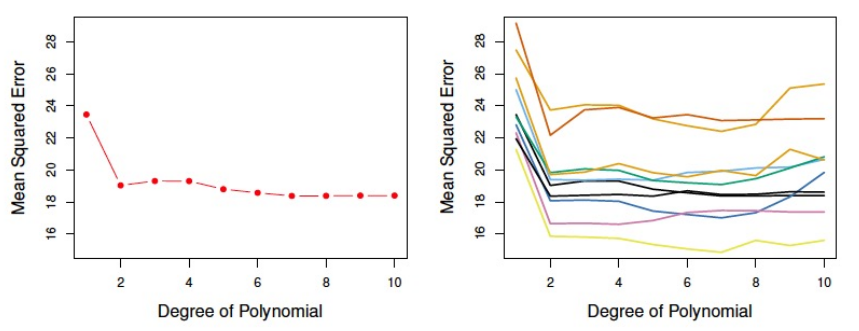
\includegraphics[width=0.8\linewidth]{./figures/chapter_4/lec_15_validation_set.png}
    \caption{Left: Validation error rate for a single split; Right: Validation error rate for different random splits.}
    \label{fig:lec_15_validation_set}
\end{figure}

As we can see from the plots above, there is a lot of variability among the MSE if we change the training/validation set. The results obtained don't agree on a particular degree. 

In fact, we can state that the validation set approach has two main drawbacks:
\begin{itemize}
    \item the validation MSE can be highly variable, depedening on the observations included in the training set and the validation set. 
    \item only a subset of the observations are used to fit the model, reducing the data used to train the model. This can lead into an overestimation of the test error.
\end{itemize}
To overcome these two drawbacks, a \textbf{cross-validation} technique is often used.

\subsubsection*{Leave-One-Out Cross-Validation}
As the validation set approach, the \textbf{leave-one-out cross-validation} (LOOCV) expect the split of the data in two parts. 
The first one is a validation set made by a single observation $(x_i, y_i)$, and the second one is the training set made by all the other observations. The model is fitted on the training set and the resulting model is used to predict the response for the single observation in the validation set.
This procedure is repeated $n$ times, each time leaving out a different observation. 

The LOOCV estimate for the test error is the average of these $n$ test error estimates.

% Split the data ${(x_i, y_i)}$ into a validation set $(x_1,y_2)$ and a training set $(x_2, y_2, \dots, x_n, y_n)$. Fit the model on the training set and validate the model using the validation set, computing the corresponding \textit{test error} MSE. Repeat this procedure $n$ times, each time leaving out a different observation. The LOOCV estimate for the test MSE is the average of these $n$ test error estimates.
\[
    CV_{(n)} = \frac{1}{n} \sum_{i=1}^{n} MSE_i
\]

The LOOCV approach has a number of desirable properties:
\begin{itemize}
    \item it has far less bias than the validation set approach, since we repeatedly fit the model using a training set that contains $n-1$ observations, almost as many as are in the entire data set.
    \item it produces a less variable MSE estimate, since there is no randomness in data splits. For this reason, by applying several times the LOOCV we obtain the same result.
\end{itemize}

The main issues with this method is that it can be computationally expensive, because each model is fit $n$ times, especially for a very large dataset.

\subsubsection*{k-Fold Cross-Validation}
The idea behind the k-fold cross validation is to randomly divide the data into $K$ equal-sized parts. We leave out part $k$, fit the model to the other $K-1$ parts and then obtain predictions for the left-out $k$th part. This is done in turn for each part $k = 1, \dots, K$, and then the results are averaged.

Let the $K$ parts be $C_1, \dots, C_K$, where $C_k$ denotes the indices of the observations in the $k$th part. There are $n_k$ observations in part $k$, if $n$ is a multiple of $K$ then $n_k = \frac{n}{K}$.

We compute:
\[
    CV_{(K)} = \frac{1}{K} \sum_{k=1}^{K} MSE_k = \frac{1}{K} \sum_{k=1}^{K} \frac{1}{n_k} \sum_{i \in C_k} (y_i - \hat{y}_i)^2
\]
%TODO: qua credo ci fosse un errore nel definire \hat y_i. per cui commento e correggo, ma da chiedere a Miriam
% Where $MSE_k$ is the mean squared error for the $k$th part, and $\hat{y}_i$ is the prediction obtained from the fit of the model to the $k$th part, excluding observation $i$.
Where $MSE_k$ is the mean squared error for the $k$th part, and $\hat{y}_i$ is the prediction obtained from the fitted onto the $i$-th observation of the $k$-th part.
\begin{figure}[ht]
    \centering
    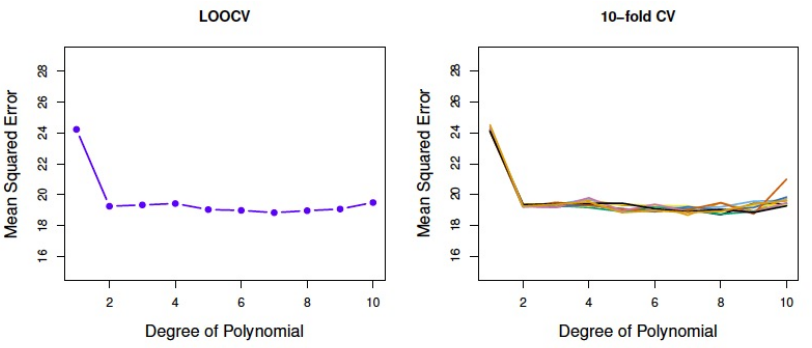
\includegraphics[width=0.8\linewidth]{./figures/chapter_4/lec_15_k_fold_cv.png}
    \caption{Left: LOOCV error curve; Right: 10-fold CV error curves.}
    \label{fig:lec_15_k_fold_cv}
\end{figure}
As we can see in the plots above, if we repeat the $k$-fold cross validation with different splits we obtain different MSE, but the variance is lower than the validation set approach. 

Both the LOOCV and the $k$-fold CV methods tend to give similar results, they are both stable and produce similar MSE estimates.

\paragraph*{Bias-Variance Trade Off for $k$-fold CV}
When used with $k < n$, the $k$-fold CV method has a computational advantage over LOOCV, and gives more accurate estimates of the test error rate with respect to LOOCV, this is because of the \textbf{bias-variance trade-off}.

\subparagraph*{Bias} 
Typically the validation set approach leads to an overestimation of the test error, because we use a training set that is smaller than the actually one. Instead, for the very same reason, the LOOCV provides approximatively unbiased estimates of the test error, due to the fact that the model is fitted using a training set that contains $n-1$ observations, almost as many as are in the entire data set. For what concerns the $k$-fold CV, when used with $K=5$ or $K=10$, it provides a trade-off between the computational expense of LOOCV and the potential bias of the validation set approach, because the model is fitted using a training set that contains $(K-1) \frac{n}{k}$ observations (less thant LOOCV but more than validation set approach).

\subparagraph*{Variance}
In an estimation procedure also the variance of the estimate is important.

Since in the LOOCV we are averaging the outputs of $n$ fitted models, each of which is trained on an almost identical set of observations, with high correlation with each other. Instead, using $k$-fold CV we are averaging the outputs of $K$ fitted models that are trained on less correlated sets of observations, because the overlap between the training set is smaller. The mean of many highly correlated quantities has higher variance with respect to the mean of many quantities that are not highly correlated. So, the test error estimate resulting from LOOCV has higher variance with respect to the test error estimate resulting from $k$-fold CV.

We can resume by saying that, in the general case of $k$-fold CV, the bias-variance trade-off is dictated by the choice of $K$. The more we increase $K$, the more we reduce the bias of the test error estimate, but the more we increase the variance of the test error estimate. Empirically, it has been shown that $K=5$ or $K=10$ is a good compromise.
% \paragraph*{LOOCV vs K-Fold CV}
% K-fold CV with $K < n$ has a computational advantage over LOOCV, and gives \textit{more accurate estimates} of the \textit{test error} rate with respect to LOOCV, this is because of the \textbf{bias-variance trade-off}.

% \textbf{LOOCV} has \textit{less bias} but \textit{higher variance} than $K$-fold CV. The bias is smaller because LOOCV uses a training dataset containing $n-1$ samples while k-fold uses a training dataset containing $(K-1) \frac{n}{k}$. The variance is higher because LOOCV averages the outputs of $n$ fitted models each of which is trained on an almost identical set of observations, highly correlated with each other, by contrast in K-fold CV we are averaging the outputs of $K$ fitted models that are trained on less correlated sets of observations, because the overlap between the training set is smaller.\footnote{The mean of many highly corrlated quantities has higher variance with respect to the mean of many quantities that are not highly correlated.}

% In conclusion, most of the times we use $K$-fold CV with $K=5$ or $K=10$, because it has been shown empirically that it suffer neither from excessively high bias nor from very high variance.

\subsection*{Bootstrap}
The \textbf{bootstrap} method is used to quantify the uncertainty associated with a given estimator. For example, it can provide an estimate of the standard error of a coefficient, or a confidence interval for that coefficient. The main advantage is the fact it can be easily applied to a wide range of statistical learning methods, including some for which a measure of variability is otherwise difficult to obtain.

\paragraph*{Example}
Suppose we wish to invest a fixed sum of money in two financial assets that yield returns of $X$ and $Y$, where $X$ and $Y$ are random variables.

We will invest a fraction $\alpha$ of our money in $X$ and will invest the remaining $1-\alpha$ in $Y$. We wish to choose $\alpha$ to minimize the total risk or \textit{variance} of our investment.

The \textbf{variance} of our investment is given by:
\[
    \sigma^2 = \var{\alpha X + (1-\alpha)Y}
\]
We want the value of $\alpha$ that minimizes $\sigma^2$. The value of $\alpha$ that minimizes $\sigma^2$ is given by:
\[
    \alpha^\ast  = \arg\min_{\alpha} \var{\alpha X + (1-\alpha)Y} = \arg\min_{\alpha} \left(\alpha^2 \sigma^2_X + (1-\alpha)^2 \sigma^2_Y + 2\alpha(1-\alpha)\sigma_{XY}\right)
\]
Compute it by taking the derivative of the expression with respect to $\alpha$ and setting it equal to zero, we obtain: %TODO: possiamo esplicitare il calcolo?
\[
    \alpha = \frac{\sigma^2_Y - \sigma_{XY}}{\sigma^2_X + \sigma^2_Y - 2\sigma_{XY}}
\]
The problem is that the variances and covariances are unknown, so we cannot compute $\alpha$. We can compute estimates of these quantities using a dataset that contains past measurements for $X$ and $Y$ and then use these estimates to compute $\hat{\alpha}$.
\[
    \hat\alpha = \frac{\hat\sigma^2_Y - \hat\sigma_{XY}}{\hat\sigma^2_X + \hat\sigma^2_Y - 2\hat\sigma_{XY}}
\]
\begin{figure}[ht]
    \centering
    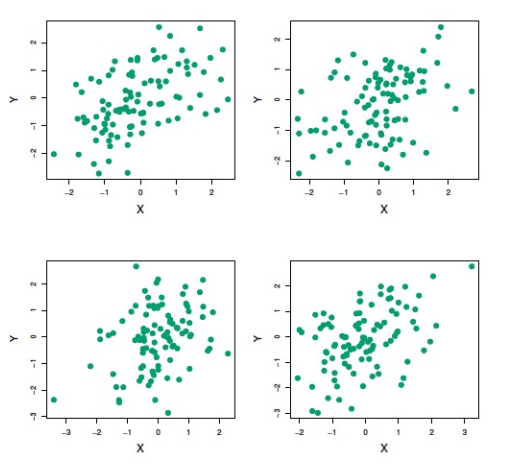
\includegraphics[width=0.8\linewidth]{./figures/chapter_4/lec_15_investment_simulations.png}
    \caption{Each panel displays 100 simulated returns for investments $X$ and $Y$, each of them gives a different estimate of $\alpha$.}
    \label{fig:lec_15_bootstrap_example}
\end{figure}

Let's imagine simulating this experiment, obtaining small datasets containing $100$ pairs representing the return on investment in $X$ and $Y$. We use this data to estimate $\sigma^2_Y$, $\sigma^2_X$ and $\sigma_{XY}$ and consequently make an estimate of $\hat \alpha$ for each of the datasets.
We would quantify the accuracy of the estimate of $\alpha$ by computing the standard deviation of the $\hat{\alpha}$ estimates. This can be done by repeating the process of simulating the data set many times, each time recomputing $\hat{\alpha}$.
In this way, if repeat the process $1000$ times, we obtain $1000$ estimates for $\alpha$ which we can call $\hat{\alpha}_1, \hat{\alpha}_2, \dots, \hat{\alpha}_{1000}$.
% To estimate the standard deviation of $\hat{\alpha}$ we repeated the process of simulating the data set of 100 paired observations of $X$ and $Y$ many times, each time recomputing $\hat{\alpha}$. This gave us $1000$ estimates for $\alpha$ which we can call $\hat{\alpha}_1, \hat{\alpha}_2, \dots, \hat{\alpha}_{1000}$.

% For these simulation the parameters were $\sigma_X^2 = 1$, $\sigma_Y^2 = 1.25$, $\sigma_{XY} = 0.5$ and thus $\alpha=0.6$.

Using these data we can compute mean and standard deviation of the $\hat{\alpha}$ estimator.
\[
    \bar \alpha = \frac 1{1000}\sum_{r=1}^{1000} \hat{\alpha}_r = 0.5996
\]
\[
    SE(\hat \alpha) = \sqrt{\frac 1{1000-1}\sum_{r=1}^{1000} \left(\hat{\alpha}_r - \bar{\alpha}\right)^2} = 0.083
\]
So, we can say that the estimate $\hat\alpha$ will differ from the true value of $\alpha$ by approximately $0.083$ on average.

\paragraph*{Bootstrap}
For real data we cannot generate new samples from the original population, as we did in the last experiment. The bootstrap approach allow us to mimic the process of obtaining new data sets, so that we can estimate the variability of our estimate without generating additional samples.

Rather than repeatedly obtaining independent data sets from the population, we instead obtain distinct data sets by repeatedly sampling observations from the original data set with replacement.

Each of these data sets is of the same size as the original data set. As a result, some observations may appear more than once in a given bootstrap data set and some not at all.

\begin{figure}[ht]
    \centering
    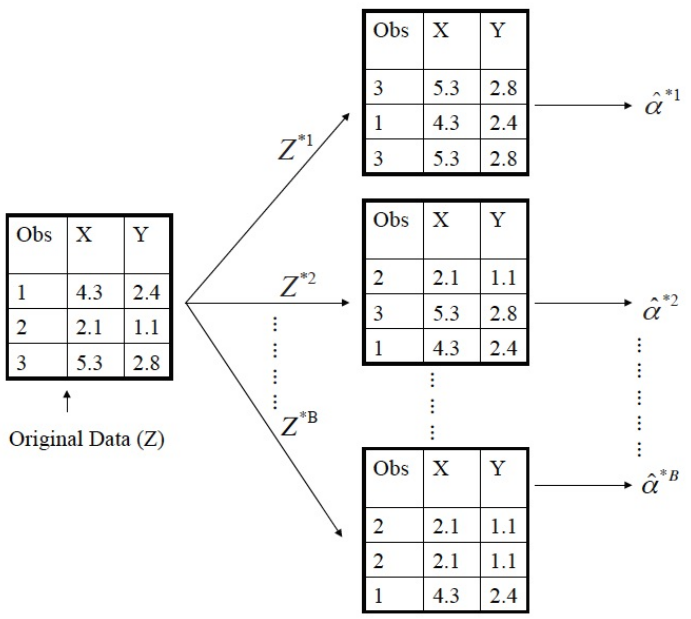
\includegraphics[width=0.8\linewidth]{./figures/chapter_4/lec_15_bootstrap.png}
    \caption{Example of bootstrap procedure.}
    \label{fig:lec_15_bootstrap}

\end{figure}

Denoting the first bootstrap data set by $Z^{\ast 1}$, we use it to produce a new bootstrap estimate for $\alpha$, which we call $\hat{\alpha}^{\ast 1}$. This procedure is repeated $B$ times for some large value of $B$, in order to produce $B$ different bootstrap data sets, $Z^{\ast 1}, Z^{\ast 2}, \dots, Z^{\ast B}$, and $B$ corresponding $\alpha$ estimates, $\hat{\alpha}^{\ast 1}, \hat{\alpha}^{\ast 2}, \dots, \hat{\alpha}^{\ast B}$.

The standard error is given by the formula below:
\[
    SE_B(\hat{\alpha}) = \sqrt{\frac{1}{B-1} \sum_{r=1}^{B} \left(\hat{\alpha r} - \frac{1}{B} \sum_{r^{\prime} =1}^{B} \hat{\alpha}^{\ast r^{\prime} }\right)}
\]
This serves as an estimate of the standard error of $\hat{\alpha}$.

In the investement example, we can use the bootstrap to estimate a standard error of $\hat{\alpha}$. Doing it we obtained an estimate of $0.087$ which is very close to the value of $0.083$ obtained from the simulation.

\begin{figure}[ht]
    \centering
    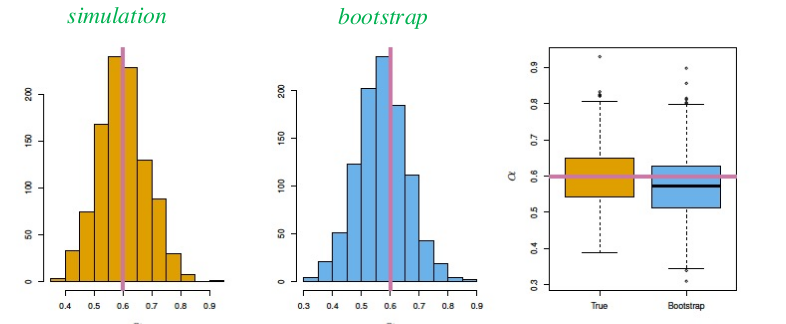
\includegraphics[width=0.8\linewidth]{./figures/chapter_4/lec_15_bootstrap_2.png}
    \caption{Comparison between bootstrap and simulation.}
    \label{fig:lec_15_bootstrap_2}

\end{figure}

In more complex situations, figuring out the appropriate way to generate bootstrap samples can require some thought. For example, if the data is a \textit{time series} we cannot simply sample the observations with replacement, but we can instead create blocks of consecutive observations and then sample those with replacements. Then we paste together the blocks to obtain a bootstrap data set.

% caption

% didn't understand this part
The bootstrap approach is primarily used to obtain standard errors of an estimate. It also provides approximate confidence intervals for a population parameter, which represents an approximate $90\%$ confidence interval for the true $\alpha$ and it is called \textbf{bootstrap percentile} confidence interval.

It is the simplest method (among many approaches) for obtaining a confidence interval from the bootstrap.

\subsection*{Final Remarks}
If we have many data, the best approach for both problems is to randomly divide the dataset into three parts called \textit{training set}, \textit{validation set} and \textit{test set}.

\begin{itemize}
    \item the \textbf{training set} is used to fit the models
    \item the \textbf{validation set} is used to estimate prediction error and perform model selection
    \item the \textbf{test set} is used for assessment of the generalization error of the final chosen model
\end{itemize}

Ideally, the test set should be brought out only at the end of the data analysis. If instead we used the test-set repeatedly and select the model with the smallest test-set error, we will underestimate the true test error.

Tipically, we use $50\%$ of the data for training, $25\%$ for validation and $25\%$ for testing. However, there are many situation in which there is insufficient data to split it into three parts. In this case, the dataset is typically split in two parts called training and test parts.

In these circumstances, the validation step is approximated either anaylitically using AIC and BIC or by using resampling methods.

\section{Model Selection}
The standard linear model is commonly used to describe the relationship between a response $Y$ and a set of predictors $X_1, \dots, X_p$. This model is typically fit using least squares which may not work well for large $p$ or in presence of multicollinearity.

There are two reasons we might not just use the ordinary least squares estimates, that are \textit{prediction accuracy} and \textit{model interpretability}.

\paragraph*{Prediction accuracy} 
If the true relationship between the response and the predictors is approximately linear, the least squares estimates will have low bias. However, we have to consider the following cases:
\begin{itemize}
    \item If $n \gg p$, meaning that if the number of observation is much larger than the number of variables, then the least squares estimates tend to also have low variance and will perform well on test observations.
    \item If $n \simeq p$, then the least squares fit can have high variance and may result in overfitting and poor estimates on unseen observation.
    \item When $n < p$ then there is no longer a unique least squares coefficient estimate, since the variance is infinite so the method cannot be used at all.
\end{itemize}

\paragraph*{Model Interpretability} 
In addition, when we have a large number of predictors $X$ in the model, there will be many of them that have little or no effect on $Y$, this reduces the \textbf{model interpretability}. Leaving these variables in the model makes it harder to see the real relationships among predictors and the dependent variable and it is difficult to appreciate the effect of the \textit{relevant variables} describing $Y$. The model would be easier to interpret by removing the unimportant variables.

\subsection{Alternative fitting procedures}
There are three different approaches that we can use to prevent this problems:
\begin{itemize}
    \item \textbf{subset selection}, in which we identify a subset of the $p$ predictors that we believe to be related to the response, we then fit a model using the least squares on the reduced set of variables.
    \item \textbf{shrinkage}, in which we fit a model involving all $p$ predictors but the estimated coefficient get shrunken towards zero. This techniques reduces variance and can perform variable selection.
    \item \textbf{dimension reduction}, in which we project the $p$ predictors into a $M-$dimensional subspace. This is achieved computing $M$ different linear combinations or projections of the variables. This $M$ projects are used as predictors to fit a linear regression model using OLS.
\end{itemize}

\subsubsection*{Subset Selection}
There are four different kinds of algorithms that implement the \textbf{subset selection} approach:
\begin{itemize}
    \item \textbf{best subset selection}
    \item \textbf{forward stepwise selection}
    \item \textbf{backward stepwise selection}
    \item \textbf{hybrid approach}
\end{itemize}

\paragraph*{Best Subset Selection}
In this approach, we run a linear regression for each possibile combination of the $X$ predictors. In order to select the "best" model, one simple apporach is to take the subset with the smallest \textit{RSS} or equivalently the largest $R^2$.

Unfortunately, the model that includes all the variables will always have the largest $R^2$ and the smallest \textit{RSS}, since these quantities are related to the training error. For this reason, we have to consider other measures to select the best model that depends on an estimate of the test error.
In order to select the best model with respect to the test error, we need to estimate this test error. There are two possible approaches:
\begin{enumerate}
    \item Estimate test error by making an \textit{adjustement} to the training error to account for the bias due to overfitting. We can use measurements such as: $C_p$, $AIC$, $BIC$, and adjusted $R^2$. These methods add a penalty to RSS for the number of variables in the model.
    \item We can \textit{directly} estimate the test error, using a validation set or a cross-validation approach.
\end{enumerate}


The algorithm for best subset selection is defined by algorithm \ref{alg:best_subset_selection}.
\begin{algorithm}[h]
    \begin{enumerate}
        \item Let $\mathcal{M}_0$ denote the \textit{null model}, which contains no predictors. This model simply predicts the sample mean for each observation.
        \item For $k = 1,2,\dots, p-1$:
        \begin{enumerate}
            \item Fit all $\binom{p}{k}$ models that contain exactly $k$ predictors.
            \item Pick all the best among these $\binom{p}{k}$ models, and call it $\mathcal M_{k}$. Here best is defined as having the smallest RSS, or equivalently largest $R^2$.
        \end{enumerate}
        \item Select a single best model from among $\mathcal{M}_0, \dots, \mathcal{M}_p$ using validation set approach, cross-validated prediction error, $C_p$, AIC, BIC or adjusted $R^2$.
    \end{enumerate}
    \label{alg:best_subset_selection}
    \caption{Best Subset Selection algorihtm}
\end{algorithm}

This algorithm can be used for other types of models not based on least squares regression, such as \textit{logistic regression}.

\paragraph*{Stepwise Selection}
The best subset selection approach is computationally infeasible for large $p$. Moreover, a large search space can lead to overfitting and high variance of the coefficient estimates. For these reasons, we usually adopt \textit{stepwise methods} that explore a smaller set of models.

The \textbf{forward stepwise selection} and \textbf{backward stepwise selection} are two common stepwise methods. The \textbf{forward stepwise selection} starts with the null model and adds the "best" predictor to the model at each step. The \textbf{backward stepwise selection} starts with the full model and removes the "worst" predictor at each step. Both of them fit a total of $p(p+1)/2 + 1$ models that is substantially better than $2^p$. These two methods are defined by algorithms \ref{alg:forward_stepwise_selection} and \ref{alg:backward_stepwise_selection}.
\begin{algorithm}
    \begin{enumerate}
        \item Let $\mathcal M_0$ be the \textit{null model}, i.e. it does not contain any predictors
        \item For $k=0,1,\dots,p-1$:
        \begin{enumerate}
            \item Consider all $p-k$ models that increase the number of predictors in $\mathcal M_k$ with an additional predictor
            \item We choose the best among these $p-k$ models, we call it $\mathcal M_{k-1}$. Here best means the model that optimizes $RSS$ or $R^2$.
        \end{enumerate}
        \item We select a single best model among $\mathcal M_0,\dots,\mathcal M_p$ using the prediction error on the validation set, or techniques like $C_p$ $(AIC)$, $BIC$, or $ AdjR^2$. Alternatively we can also use the cross validation method.
    \end{enumerate}
    \caption{Forward Stepwise Selection}
    \label{alg:forward_stepwise_selection}
\end{algorithm}

\begin{algorithm}
    \begin{enumerate}
        \item Let $\mathcal M_p$ be the \textit{full model}, i.e. it contains all the $p$ predictors
        \item For $k=p,\dots,1$:
        \begin{enumerate}
            \item Consider all $k$ models that contain all but one of the predictors in $\mathcal M_k$, for a total of $k-1$ predictors
            \item We choose the best among these $k$ models, we call it $\mathcal M_{k-1}$. Here *best* means the model that optimizes $RSS$ or $R^2$.
        \end{enumerate}
        \item We select a single best model among $\mathcal M_0,\dots,\mathcal M_p$ using the prediction error on the validation set, or techniques like $C_p$ $(AIC)$, $BIC$, or $ AdjR^2$. Alternatively we can also use the cross validation method.
    \end{enumerate}
    \caption{Backward Stepwise Selection}
    \label{alg:backward_stepwise_selection}
\end{algorithm}

Certainly, the forward stepwise selection and the backward stepwise selection are not guaranteed to find the best model out of all $2^p$ models. However, they are much faster than the best subset selection and they are more stable.

Another interesting aspect is that the forward stepwise selection can be used when $n < p$, while the backward stepwise selection cannot be used in this case.

Forward stepwise and backward stepwise selection return similar models in general, but not identical. An alternative to them is the \textbf{hybrid approach}, which is a combination of the two methods. It starts with no predictors and at each step adds the best predictor among all the predictors not in the model, but can also remove a predictor at each step. This approach tries to mimic the best subset selection, but it is computationally more efficient.
\subsubsection*{Choosing the Optimal Model}
In the algorithms presented above, we have to choose the best model among $\mathcal M_0, \dots, \mathcal M_p$. Potentially, there are two different approaches to do this:
\begin{itemize}
    \item \textbf{directly estimation} with data for each model and then select the model for which the estimated test error is smallest. This can be done using the validation set approach, cross-validated prediction error.
    \item \textbf{make an adjustment} of the trainin error for estimate the test error. We can use measurements such as $C_p$, $AIC$, $BIC$, and adjusted $R^2$.
\end{itemize}

Let's see the most common methods for model selection by making an adjustment of the training error.
\paragraph*{Mallow's $C_p$}
For a fitted OLS model containing $d$ predictors, the $C_p$ estimate of test MSE is:
\[
    C_p = \frac{1}{n} \left(RSS + 2d\hat{\sigma}^2\right)
\]
where $\hat{\sigma}^2$ is an estimate of $\sigma^2 = \text{Var}(\epsilon)$. This statistics adds a penality of $2d\hat{\sigma}^2$ to the training RSS in order to adjust for the fact that the training error tends to underestimate the test error.

We can show that if $\hat{\sigma}^2$ is an unbiased estimate of $\sigma^2$, then $C_p$ is an unbiased estimate of test MSE.

\paragraph*{Akaike Information Criterion}
The AIC criterion is defined for a large class of models fit by maximum likelihood:
\[
    \text{AIC} = -2\log L + 2 \cdot d
\]
where $L$ is the maximized value of likelihood.

In the case of the linear model with Gaussian errors, maximum likelihood and least squares are the same thing. In this case AIC is given by:
\[
    \text{AIC} \propto \text{RSS} + 2d\hat{\sigma}^2
\]
Thus, for least squares models, $C_p$ and AIC are equivalent.

\paragraph*{Akaike Information Criterion}
The BIC criterion is derived from a Bayesian point of view, but ends up looking similar to $C_p$ and AIC. For the OLS model with $d$ predictors the BIC is given by:
\[
    \text{BIC} = - 2 \log L + \log(n) d
\]
which means:
\[
    BIC \propto RSS + \log (n)d \hat{\sigma}^2
\]

Since $\log n > 2$, for any $n > 7$, the BIC statistic generally places a heavier penalty on models with many variables and hence results in the selection of smaller models than $C_p$.

\paragraph*{Adjusted $R^2$}
For a least squares model with $d$ variables, the adjusted $R^2$ statistic is calculated as:
\[
    \text{adjusted } R^2 = 1 - \frac{\frac{\text{RSS}}{n-d-1}}{\frac{\text{TSS}}{n-1}}
\]
A large value of adjusted $R^2$ indicates a model with a small test error.
Unlike the other statistics presented, for which a small value indicates a model with a low test error, a large value of adjusted $R^2$ indicates a model with a small test error.

Maximizing the adjusted $R^2$ is equivalent to minimizing $\frac{\text{RSS}}{n-d-1}$. While RSS always decreases as the number of variables in the model increases, $\frac{RSS}{n-d-1}$ may increase or decrease, due to the presence of $d$ in the denominator.

Unlike the $R^2$ statistic, the adjusted $R^2$ statistic pays a price for the inclusion of unnecessary variables in the model.

$C_p$, AIC, BIC have all rigorous theoretical justifications. The adjusted $R^2$ is quite intuitive but it's not motivated in statistical theory. All of these measures are simple to compute and can serve estimates of the test error but none of then is perfect. They can also be compute in case of general types of models.

% \subsubsection*{Validation and cross-validation}

% Each of the procedures returns a sequence of models $\mathcal{M}_k$ indexed by model size $k = 0,1,2,\dots$. We need to select the best $\hat{k}$.
% We then compute the validation set error or the cross-validation error for each model $\mathcal{M}_k$ under consideration and the select the $k$ for which the resulting estimated test error is smallest.

% With respect to the previous estimates, the validation set approach provides a direct estimate of the test error without requiring the variance $\sigma^2$. This approach can also be used in a wider range of model selection tasks.

\subsubsection*{One-standard-error rule}
We usually see that the model with the lowest estimated test error has a certain number of predictors, but there isn't much difference in terms of test errors between the best model and some models with less predictors.

We can select a model using the \textbf{one-standard-error rule}, we calculate the standard error of the estimated test \textit{MSE} for each model size and then we select the smallest model for which the estimated test error is within one-standard error of the lowest point on the curve.

\begin{figure}
    \centering
    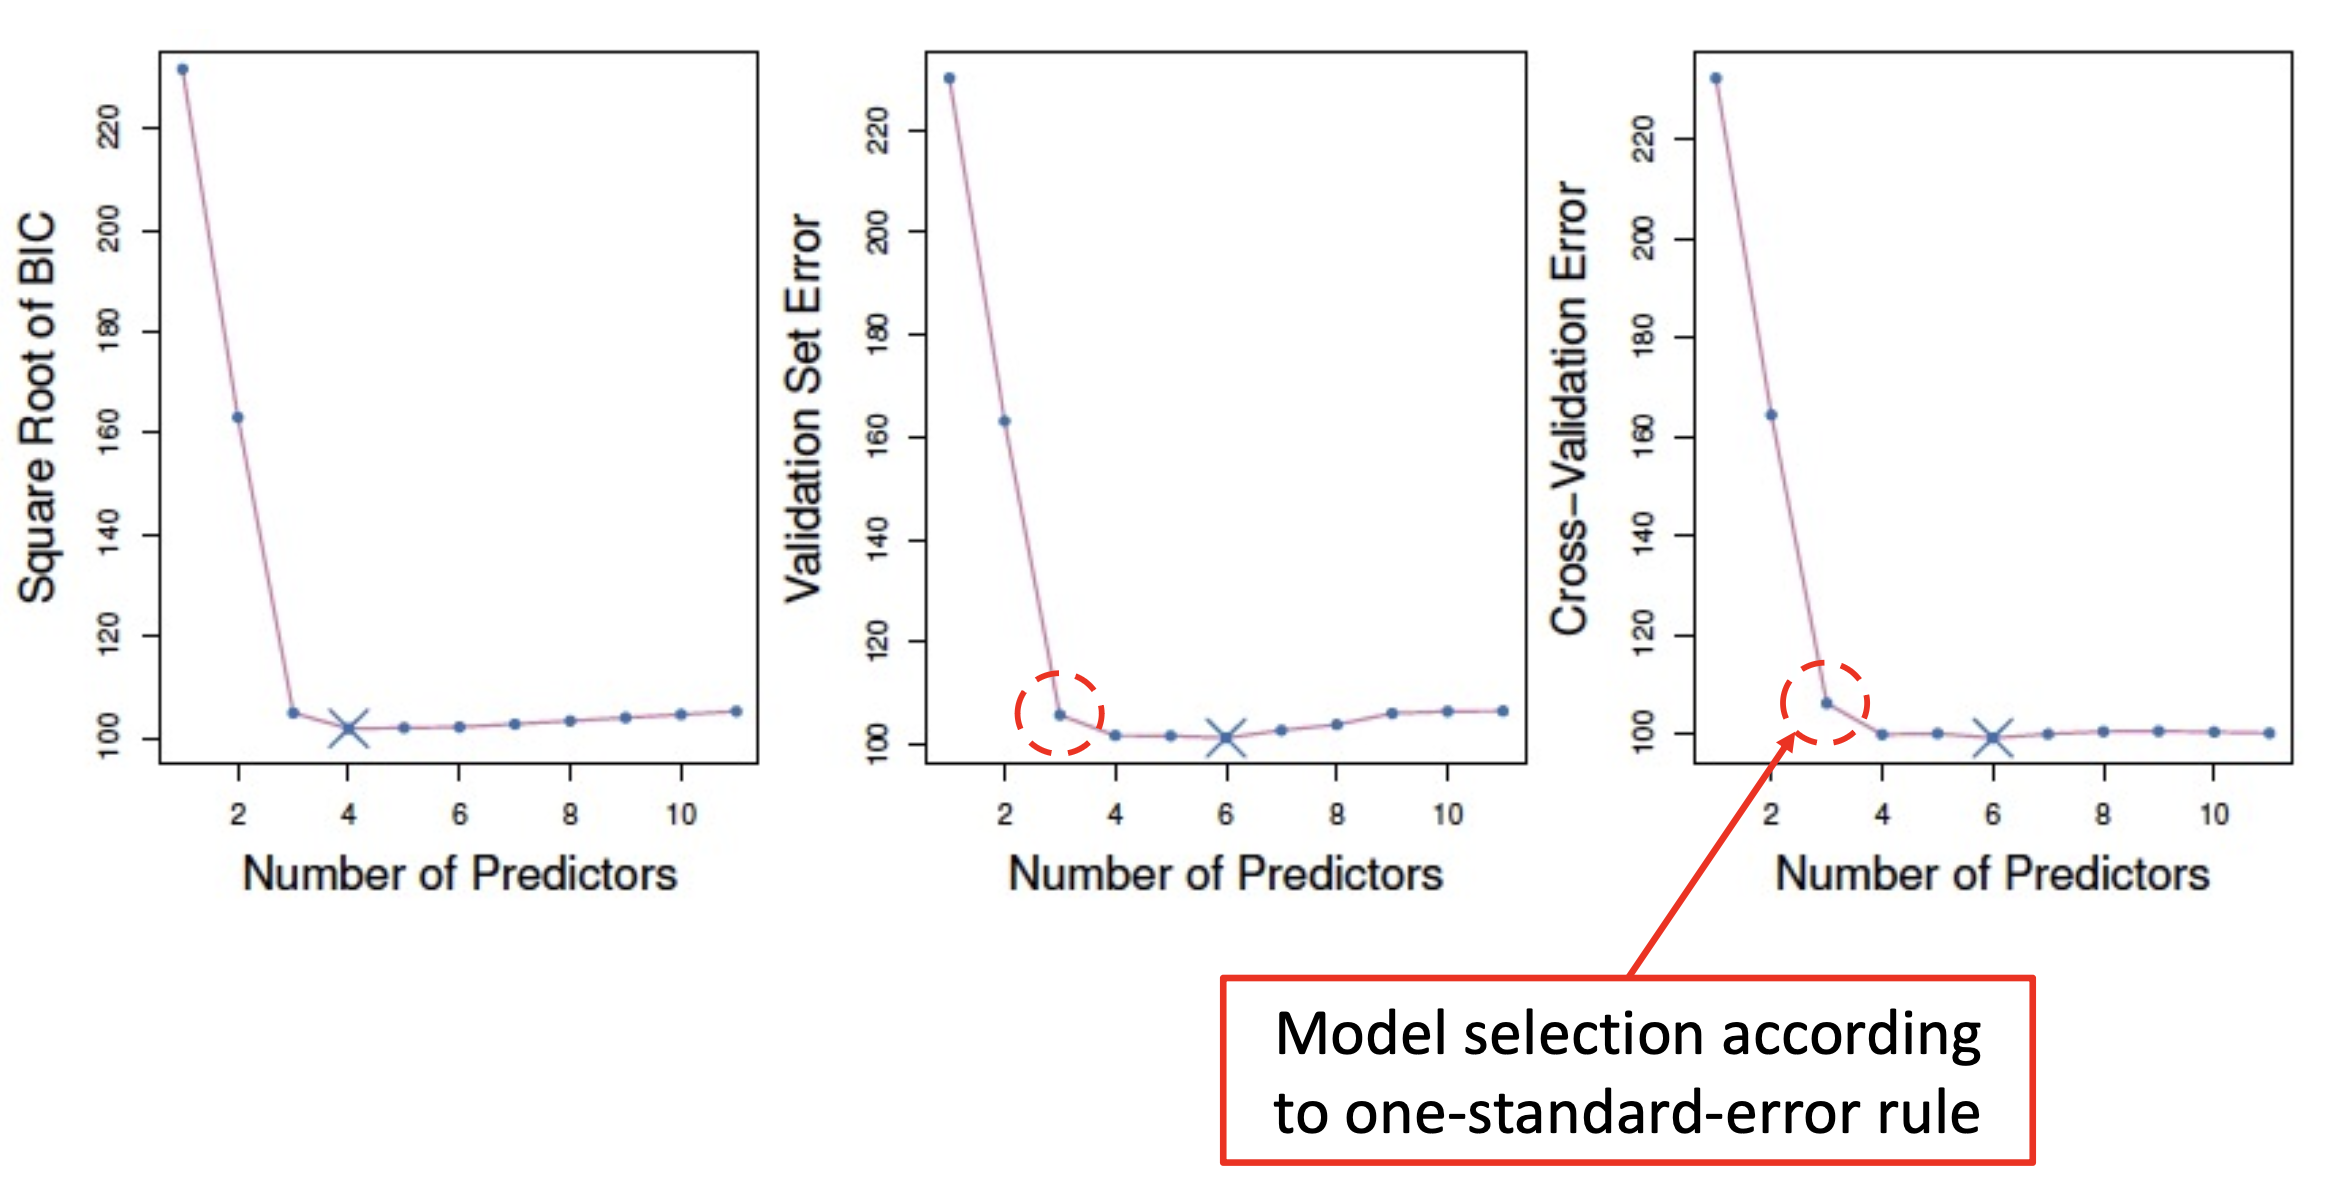
\includegraphics[width=0.8\linewidth]{./figures/chapter_4/onestandarderror.png}
    \caption{One-standard-error rule.}
    \label{fig:lec_15_one_standard_error_rule}
\end{figure}

A practical example of this rule is shown in figure \ref{fig:lec_15_one_standard_error_rule}. The plot shows the estimated test \textit{MSE} for each model size, the lowest point on the curve is the model with the smallest estimated test \textit{MSE}. The one-standard-error rule tells us to select the most parsimonious model for which the estimated test \textit{MSE} is within one standard error of the lowest point on the curve.

We can identify the following steps to apply the one-standard-error rule: %TODO: check
\begin{algorithm}
    \begin{enumerate}
        \item $\forall d$ calculate $\sigma_{\text{TestMSE}}(d)$, as standard error of the estimated test \textit{MSE} for the model with $d$ predictors.
        \item Take $\hat d$ as the number of predictor with the lowest estimated test \textit{MSE}.
        \item Identify the interval $I = [\text{TestMSE}(\hat d) - \sigma_{\text{TestMSE}}(\hat d), \text{TestMSE}(\hat d) + \sigma_{\text{TestMSE}}(\hat d)]$.
        \item Select $d^\ast = \arg\min_d[\text{TestMSE}(d) : \text{TestMSE}(d) \in I]$.
    \end{enumerate}
    \caption{One-standard-error rule algorithm}
\end{algorithm}


\section{Shrinkage Methods}
The subset selection methods use least squares to fit a linear model that contains a subset of the predictors. As an alternative we can fit a model containing all \textit{p} predictors using a technique called \textbf{shrinkage} that \textit{constraints} or \textit{regularize} the coefficient estimates towards zero.

This technique can significantly reduce the variance of the coefficients estimate at the cost of increasing the bias error.

\subsection{Ridge Regression}
Given our training data $\mathcal{D} = \{(x_i, y_i)\}_{i=1}^n $ ordinary least squares minimizes the \textit{residual sum of squares}:
\[
    \text{RSS} = \sum_{i=1}^{n} \left(y_i - \beta_0 - \sum_{j=1}^{p} \beta_j x_{ij}\right)^2
\]
The Ridge Regression approach is very similar to OLS, except that the coefficient estimates are the values that minimize:
\[
    \text{RSS'} = \sum_{i=1}^{n} \left(y_i - \beta_0 - \sum_{j=1}^{p} \beta_j x_{ij}\right)^2 + \lambda \sum_{j=1}^{p} \beta_j^2
\]
where $\lambda\ge 0$ is a tuning parameter. This additional term is called \textbf{shrinkage penalty}.

The shrinkage penalty can shrink the estimates of $\beta_j$ towards zero. We will use $\hat{\beta}^R$ to denote the coefficient estimates of the parameters $\beta$ for a fixed value of $\lambda$.
The value $\text{RSS'}$ represents a \textit{trade-off} between:
\begin{enumerate}
    \item the fit of the model to the training data, by minimizing the RSS term
    \item the magnitude of the coefficients, by minimizing the penalty term
\end{enumerate}

The tuning paramter $\lambda$ is used to enforce or reduce the shrinkage.
When $\lambda = 0$, we get the OLS estimates, whereas when $\lambda \to \infty$ the impact of the penalty term grows and the coefficient estimates will approach zero.

So, a crucial difference between ridge regression and OLS is that we get a different set of coefficient estimates for each value of $\lambda$.

Note that the shrinkage penalty \underline{is not applied to the intercept parameter $\beta_0$}, because the intercept is a \textbf{measure of the mean value of the response} when independent variables are equal to zero. 
Moreover, if we assume that the predictors $(X_{\cdot, 1}, \dots, X_{\cdot, p})$, that are simply the columns of the data matrix $\underline{\underline X}$, have been centered to have mean zero, then the intercept is the mean of the response:
\[
    \hat{\beta}_0 = \bar{y} = \frac{1}{n} \sum_{i=1}^{n} y_i
\]
%TODO: provide a justification to the previous result

\paragraph*{Example}
\begin{figure}
    \centering
    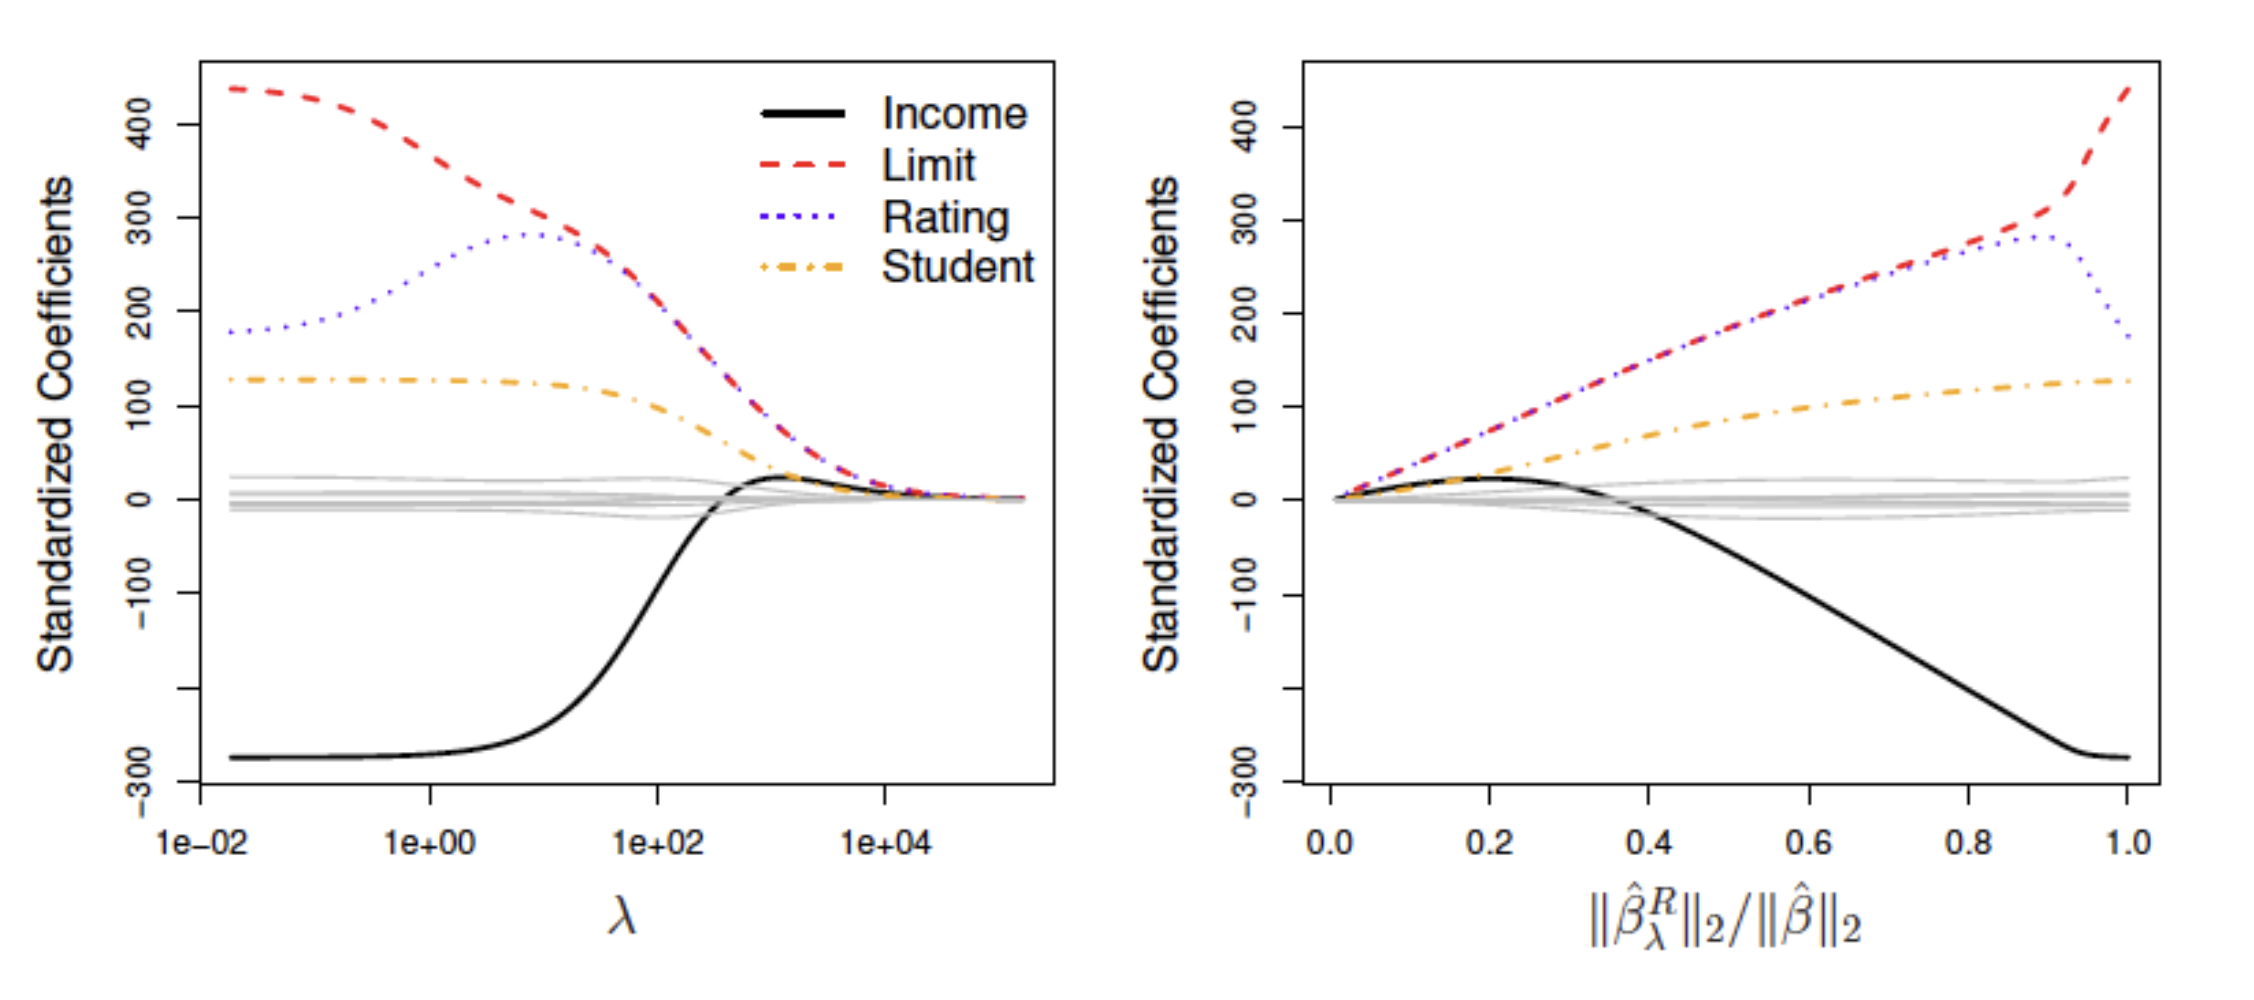
\includegraphics[width=0.8\linewidth]{./figures/chapter_4/examplecredit.png}
    \caption{Ridge regression coefficients example on Credit dataset.}
    \label{fig:examplecredit}
\end{figure}
The figure \ref{fig:examplecredit} shows an example of coefficients shrinkage on the \texttt{Credit} dataset. 

The left plot shows how the standardized ridge coefficients change as $\lambda$ varies. As we increase $\lambda$, the ridge regression coefficient estimates are shrunk towards zero, so each curve tends to be flatter than the OLS estimates. As particular case, the extreme case of $\lambda = 0$ corresponds to the OLS estimates.
The right plot, instead, shows how coefficient estimates change as the ratio between the $\ell_2$ norm of the ridge regression estimates and the OLS estimates varies. Remember that the $\ell_2$ norm of a quantity is calculated by:
\[
    \lVert \beta \rVert_2 = \sqrt{\sum_{j=1}^{p} \beta_j^2}
\]
The $\ell_2$ norm of a quantity is a measure of the distance of the quantity from the origin. 
That particular ratio varies from $1$ to $0$ by increasing $\lambda$ from $0$ to $\infty$.
This quantity tells us how much the ridge regression coefficient estimates have been shrunken towards zero wrt the OLS estimates. The less is the ratio, the more the ridge regression coefficient estimates have been shrunken towards zero.

\paragraph*{Scaling}
A property of the OLS estimates is that they are \textit{scale invariant} or \textit{scale equivariant}, which means that the we can fit the model even if the regressors have different scaling. This happens because multiplying $X_j$ by a constant $c$ means scaling the coefficient estimates by a factor of $\frac{1}{c}$, thus having the same result.

This is not true for the ridge regression estimates that can \textbf{change substantially} when multiplying a given predictor by a constant. The term $X_j \hat{\beta}_{j,\lambda}^R$ will depend not only on the value of $\lambda$ but also on the scaling of the $j$-th predictor and even the scaling of other predictors.

For these reasons, it is strongly advised to standardize the predictors before applying ridge regression:
\[
    \tilde{x}_{ij} = \frac{x_{ij} - \overline{x}_j}{s_j}
\]
Where $\overline{x}_j$ is the arithmetic mean and $s_j^2$ is the \textit{sampling variance}.

The previous standardization covers also the what we've said about the intercept. So we get:
\begin{itemize}
    \item $\beta_0 = \bar{y}$
    \item $\sigma_j = 1 \quad \forall j$
    \item Independence from the scaling of the predictors
\end{itemize}

\paragraph*{Why does ridge regression improve OLS?}
The advantage of Ridge Regression over OLS is rooted in the \textbf{bias-variance trade-off}. So as $\lambda$ grows, the flexibility of ridge regression decreases, which amounts to a decrease in terms of \textit{variance} but a growth in terms of \textit{bias}.

\begin{figure}
    \centering
    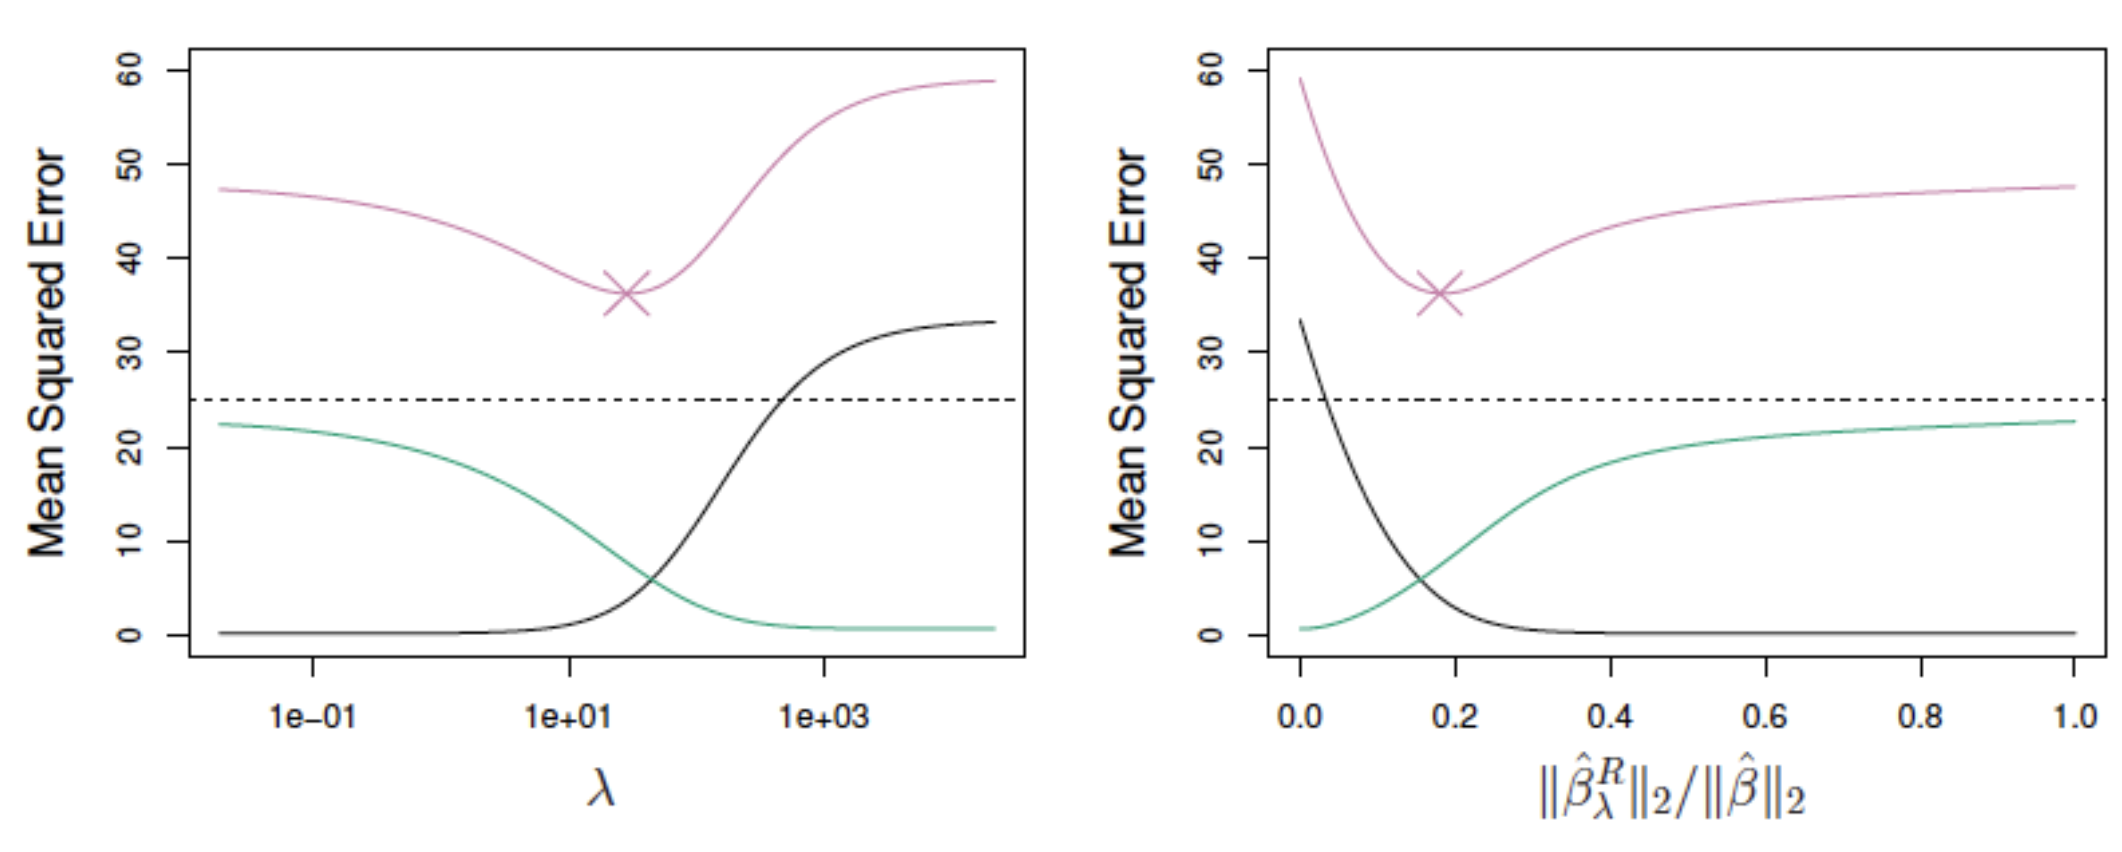
\includegraphics[width=0.8\linewidth]{./figures/chapter_4/ridgetradeoff.png}
    \caption{Ridge regression trade-off. \textcolor{green}{Green} curve represents the variance, black curve represents the bias and the \textcolor{red}{red} curve represents the test mean squared error.}
    \label{fig:ridgetradeoff}
\end{figure}

We see this in the left panel of the figure \ref{fig:ridgetradeoff}, obtained using a dataset having $p=45$ and $n=50$.

For the OLS estimates, which correspond to the leftmost point in the left panel, the variance is high but the bias is practically zero.
As we increase $\lambda$ we begin to feel the effect of shrinkage and thus the variance tends to decrease at the expense of an increase in bias.
The MSE test is proportional to alls sum between bias and variance. When $\lambda$ goes from $0$ to $10$ we notice the variance decreasing rapidly, allowing the MSE test to reach a minimum. 
Beyond this point, the variance decreases and then the shrinkage begins to be such that the estimates are underestimated and there is a large increase in bias.

\callout{Note}{In this particular example the test error that we get for the OLS estimate is not so different from the test error obtained by the null model!}

In the right panel we notice the same behavior as a function of the $\ell_2$ norm. Moving from left to right the fit becomes more flexible, decreasing the bias and increasing the variance.

\callout{Note}{In general, when the relationship between predictors and response is close to being linear, the OLS estimate will have small bias but high variance. This means that a small change in training data could lead to a large change in coefficient estimation.
This effect is especially pronounced when $p\approx n$ as in the example above. Or when one is affected by multicollinearity and similar phenomena.}

\paragraph*{Final remarks}
A final consideration that can arise is that the ridge regresssion is useful when the OLS estimates have high variance. Moreover, comparing with the \textit{Best Subset Selection}, the ridge regression is more efficient because it can be shown the computations required to estimate ridge regression for all values of $\lambda$ are almost identical to those for fitting a model using OLS and BSS.

\subsection{Least Absolute Shrinkage and Selection Operator (LASSO)}
Ridge regression does not highlights the best predictors, but it moves the less significant coefficients towards zero. Thus, this approach cannot be used to perform \textit{subset selection}, unlike BSS and the others stepwise methods do. By the way this is not a problem from the prediction accuracy point of view, but this can create difficulties in the model interpretability.

The lasso approach overcome this disadvantage. In this method, the coefficients, which we will denote with $\hat{\beta}_\lambda^L$, minimize the following quantity:
\[
    \text{RSS'} = \sum_{i=1}^{n} \left(y_i - \beta_0 - \sum_{j=1}^{p} \beta_j x_{ij}\right)^2 + \lambda \sum_{j=1}^{p} |\beta_j |
\]

The difference from ridge regression is inside the penalty term that in this case is based $\ell_1$ norm of the parameter vectors, in contrast with the $\ell_2$ norm of the ridge regression. 
As with ridge regression, the lasso regression shrinks the coefficient estimates towards zero because of the positive penalty term introduced. 
However, the $\ell_1$ penalty force some coefficient estimates to be exactly equal to zero when $\lambda$ is large enough. 
It is said that lasso yields \textit{sparse} models, that is models that involve only a subset of the variables.

\paragraph*{Example}
\begin{figure}
    \centering
    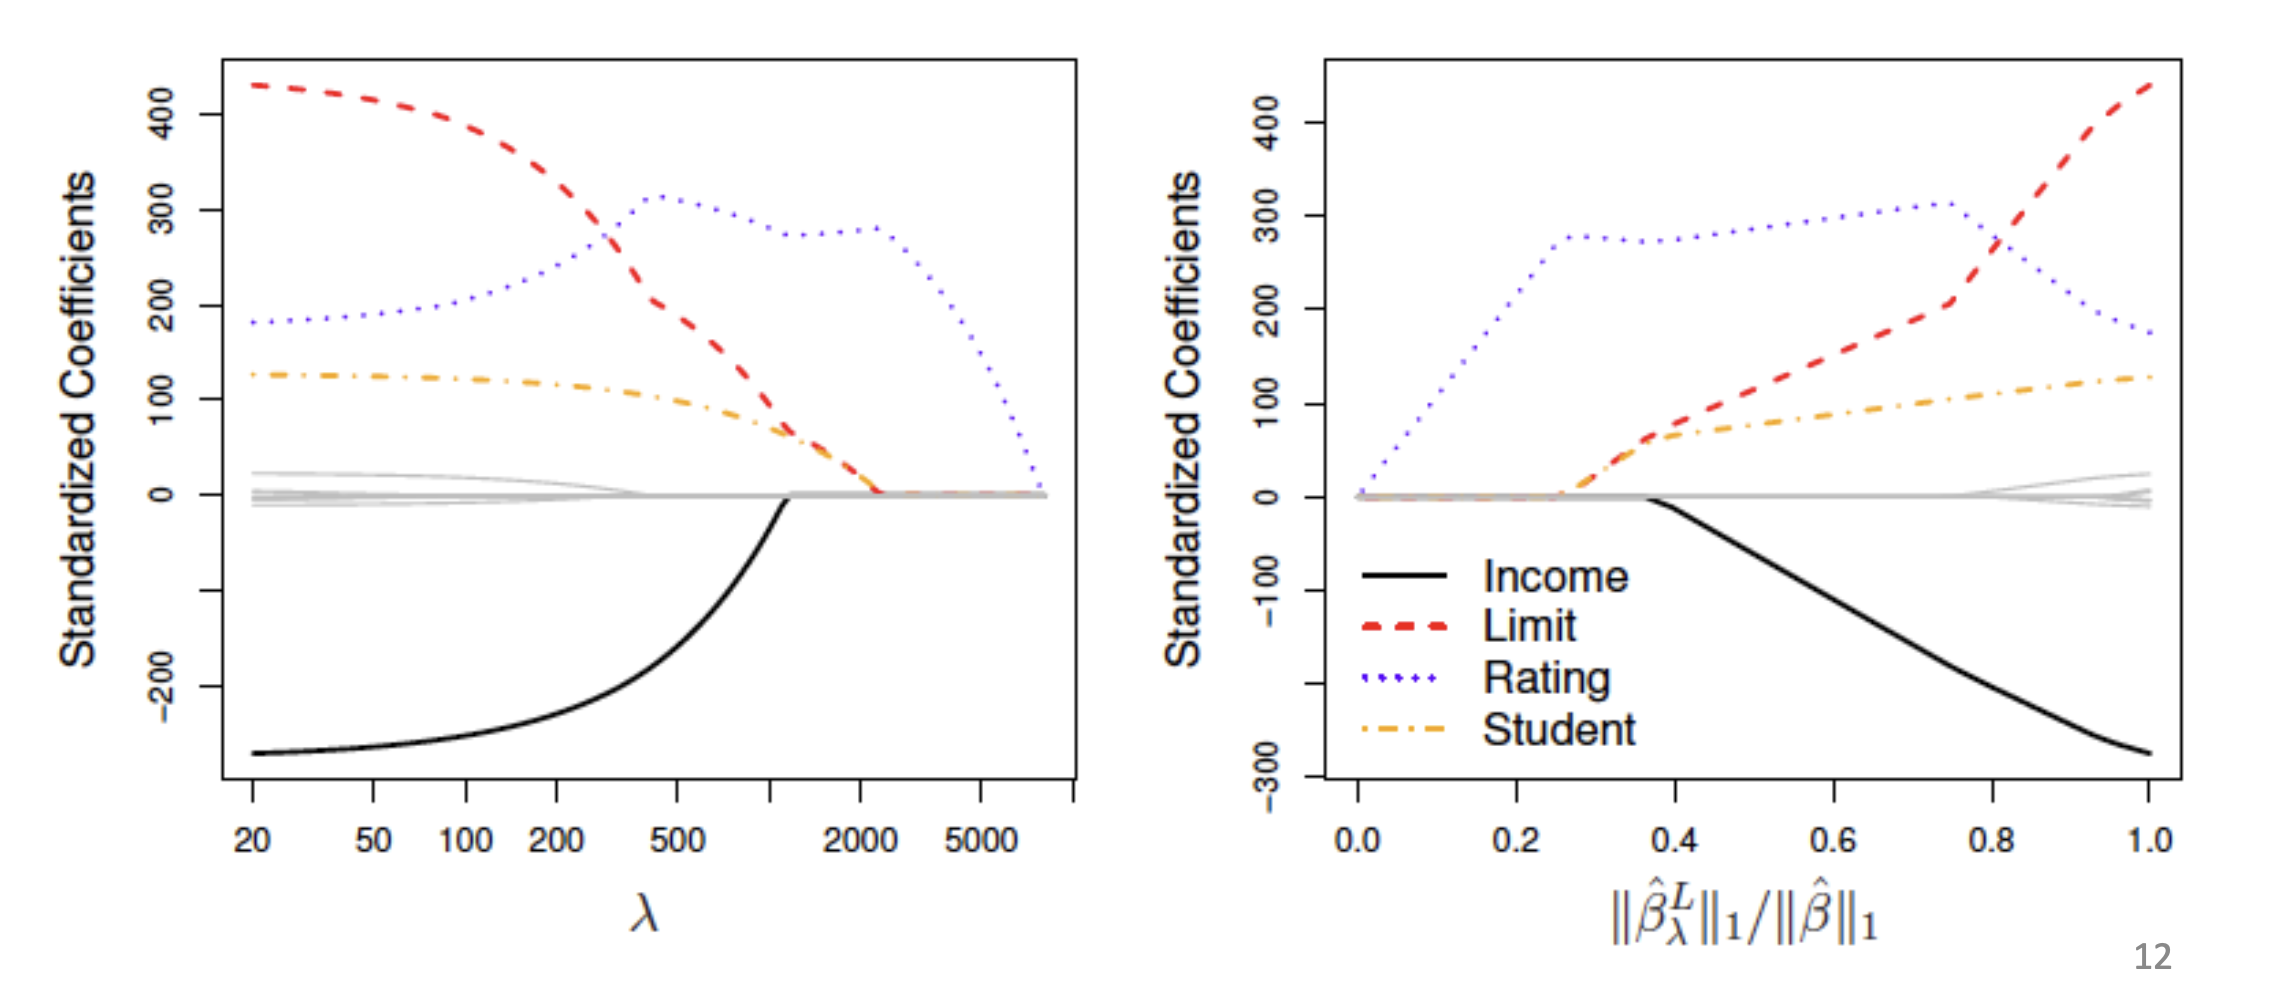
\includegraphics[width=0.8\linewidth]{./figures/chapter_4/lassoexample.png}
    \caption{Lasso regression coefficients example on Credit dataset.}
    \label{fig:lassoexample}
\end{figure}


% In order to select a good value of $\lambda$, we can employ the cross-validation approach.

The first plot shows the standardized lasso regression coefficients; here we can see that instead of converging to zero, many of the coefficients are exactly zero and this enables for model selection. 
In the final model we will remove the predictors that are zero.

The final effect of lasso is that, depending on the value of $\lambda$, we can have a model containing a number of predictors ranging from $0$ to $p$.
Ridge Regression, on the other hand, will always include all variables in the model, although their modulus will depend on $\lambda$.

\subsection*{Alternative Formulation for Ridge Regression and the Lasso}

In operational research, the minimization problems of the ridge and lasso regression are also called \textbf{dual problems}. We can get an equivalent formulation for this problem called \textbf{primal problem}.

For ridge regression the formulation requires to \textit{minimize} the following:
\[
    \text{RSS} = \sum_{i=1}^{n} \left(y_i - \beta_0 - \sum_{j=1}^{p} \beta_j x_{ij}\right)^2 \qquad \text{subject to } \sum_{j=1}^p \beta_j^2 \leq s
\]
For lasso is to minimize the following:
\[
    \text{RSS} = \sum_{i=1}^{n} \left(y_i - \beta_0 - \sum_{j=1}^{p} \beta_j x_{ij}\right)^2 \qquad \text{subject to } \sum_{j=1}^p |\beta_j| \leq s
\]
And there is also an alternative formulation for the \textit{best subset selection approach}, that is to minimize the following:
\[
    \text{RSS} = \sum_{i=1}^{n} \left(y_i - \beta_0 - \sum_{j=1}^{p} \beta_j x_{ij}\right)^2 \qquad \text{subject to } \sum_{j=1}^p I(\beta_j \neq 0) \leq s
\]
The last formulation requires us to find a set of estimates such that RSS is minimized, but with the constraint that no more than $s$ coefficient can be nonzero. The function $I(\beta_j \neq 0)$ is an \textit{indicator function} that equals $1$ if $\beta_j \neq 0$ and $0$ otherwise.

In other words, for each value of $\lambda$ there is a certain $s$ such that this optimation problem formulation will return the same estimates of the previously defined quantity. This holds for ridge coefficients, lasso coefficients and also for BSS.

Suppose that $p=2$, for visualization purposes, with that optimization problems we're saying that:
\begin{itemize}
    \item the estimates of the lasso coefficients will have the lowest RSS among all the points that lie inside a diamond-shaped constraint region defined by the equation $\|\beta_1\| + \|\beta_2\| \leq s$
    \item the estimates of the ridge coefficients will have the lowest RSS among all the points that lie inside a circular-shaped constraint region defined by the equation $\|\beta_1\|^2 + \|\beta_2\|^2 \leq s$
\end{itemize}

Moreover, that estimates, are satisfying the RSS function by knowing that there is a \textbf{budget} $s$ that we can use to fit the model. So, the constraint equation defined by the norm, must satisfy this budget.

\subsubsection*{Variable Selection property}
We've said that the lasso regression has a \textit{variable selection} property, that is, it tends to produce models that involve only a subset of the variables. This is not true for the ridge regression, which will always include all variables in the model, although their modulus will depend on $\lambda$.
We can use the optimization problem formulation in order to graphically understand that property. For this purpose we can see at the figure \ref{fig:rssregions}

\begin{figure}
    \centering
    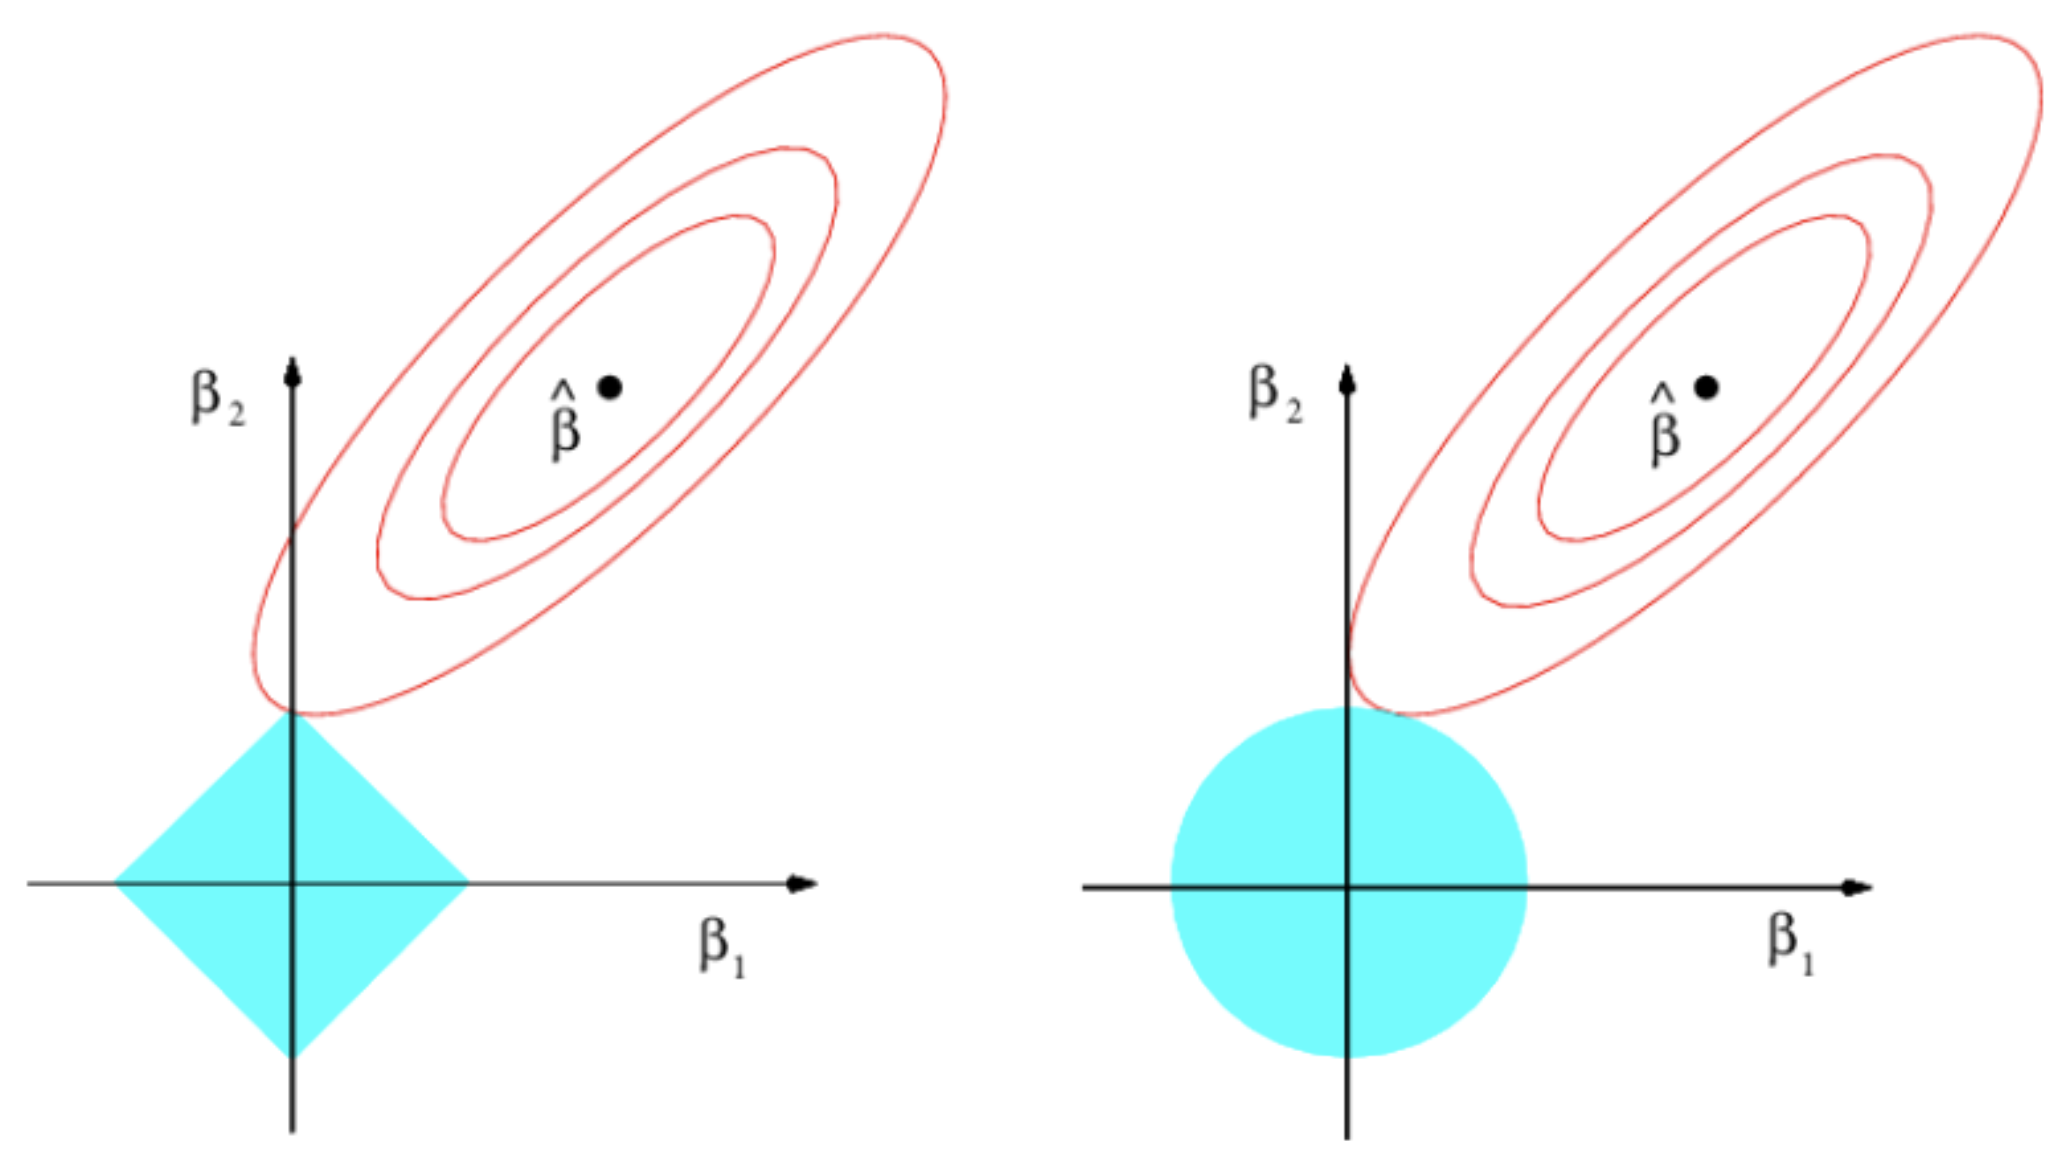
\includegraphics[width=0.8\linewidth]{./figures/chapter_4/rssregions.png}
    \caption{RSS constrained regions for lasso and ridge regression.}
    \label{fig:rssregions}
\end{figure}

The plot shows the \textit{contour plot} of the RSS in case of a model with two predictors.
The first plot shows the constraint region for the lasso approach, while the second shows the constraint region for the ridge regression.
When solving the optimization problems proposed before, we need to find the point associated to the smaller value of the RSS that lies inside the constraint regions (blue regions).

The reason why the regions are shaped like that is because by expanding the norm of the coefficients, we get the equation of a circle for the ridge regression and a diamond for the lasso regression. The constraint regions are centered at the origin and the radius of the circle or the length of the diamond's sides is determined by the value of $s$.

For a sufficient large value of $s$, the constraint regions will include the point that minimizes the RSS, and this point will be the OLS estimate. As we decrease $s$, the constraint regions will shrink and the OLS estimate will eventually lie outside of the constraint regions.
Intuitively, we also get that the value of $\lambda$ is inversely proportional to the value of $s$.

On each plot the minimum of the RSS is marked, but we can see that in this case and also in general it lies outside of the constraint regions.
The ellypses that surround the point that minimizes the RSS are \textbf{contours}, that are a collections of points that have the same value of the RSS. The optimization problems that we've defined before are saying that the coefficient estimates of lasso and ridge are given from the first point of the contour that lies inside the constraint region.

Due to the topology of the $\ell_1$ norm, it is more likely that this point will have a zero component, because that topology includes also the corners of the rectangular shape. Instead, the $\ell_2$ norm has a circular shape and the point that minimizes the RSS is more likely to be on the boundary of the constraint region. So it's more difficult to have the point on the axis.
This concept is enhanced when we have a large number of predictors, so in a high dimensional space

\subsubsection*{Comparing the Lasso and Ridge regression}
After having seen that the lasso has a variable selection property, and so the advantage to produce easier and more interpretable models, we want to compare the two methods in terms of prediction accuracy.

\begin{figure}
    \centering
    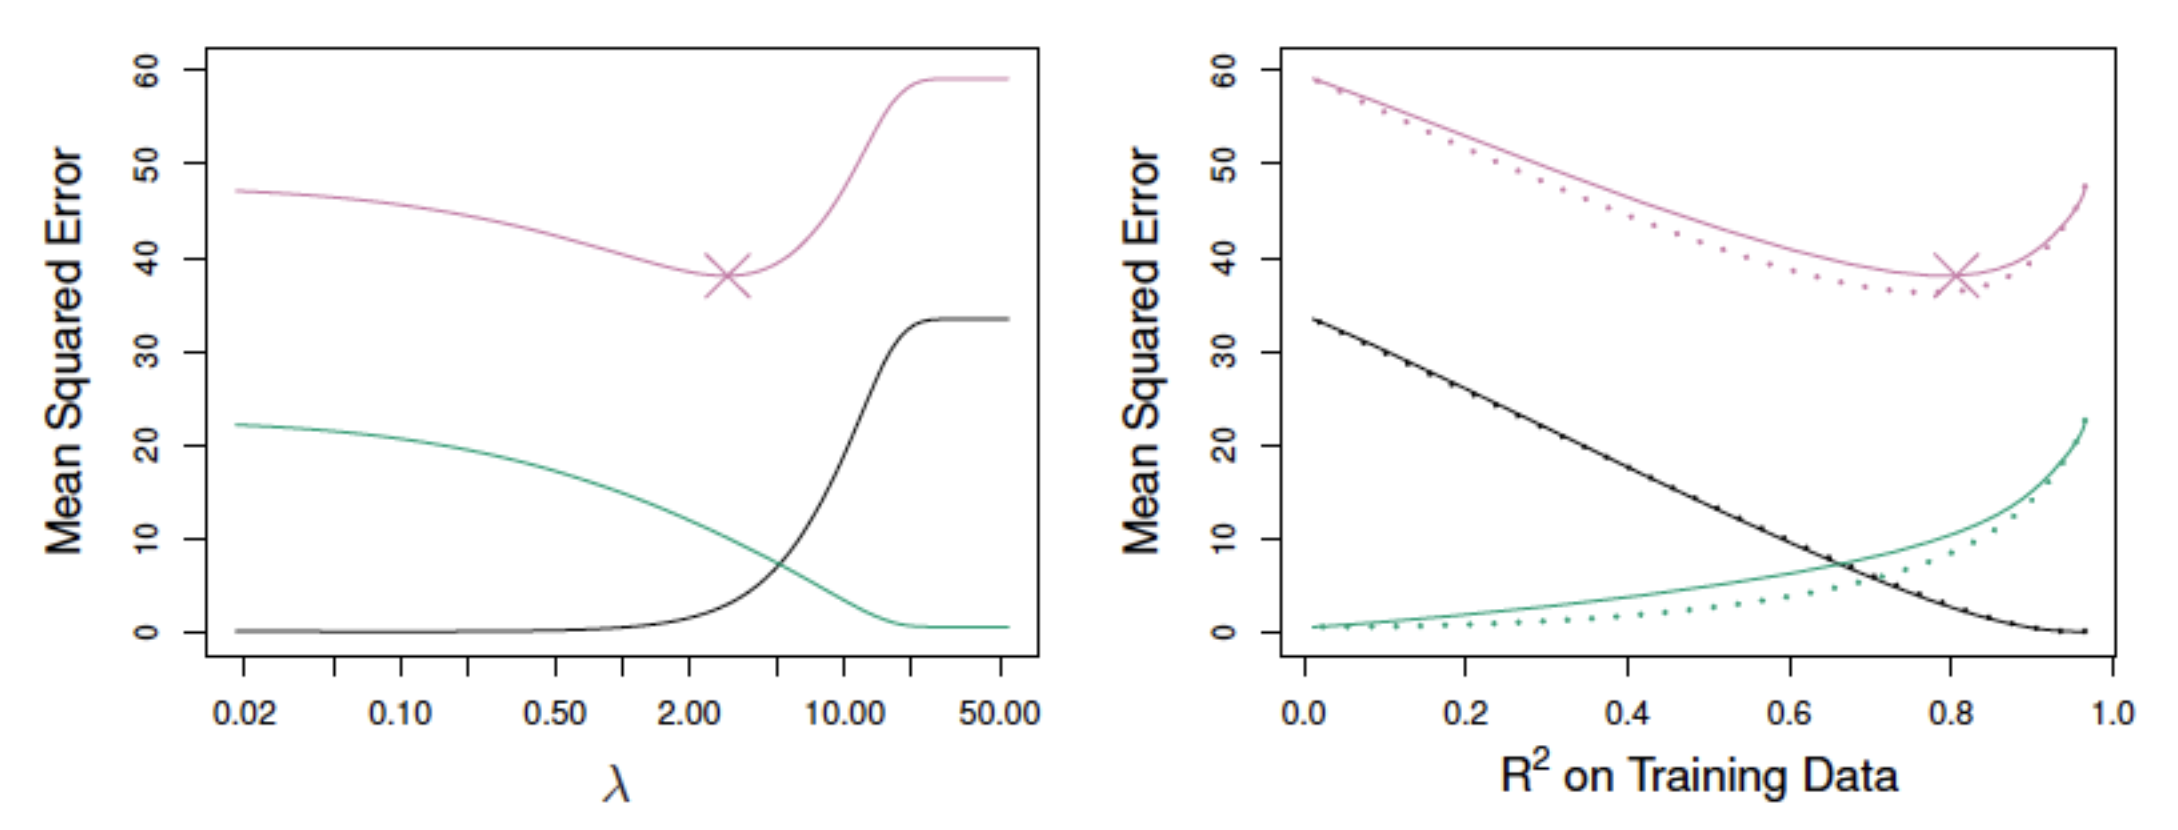
\includegraphics[width=0.8\linewidth]{./figures/chapter_4/lassoridgecomparison.png}
    \caption{Comparison between lasso and ridge regression. \textcolor{green}{Green} curve represents the variance, black curve represents the bias and the \textcolor{red}{red} curve represents the test mean squared error.}
    \label{fig:lassoridgecomparison}
\end{figure}

The figure \ref{fig:lassoridgecomparison} shows on the left plot the mean squared error and its components for lasso regression as we've already seen for ridge. While, the right plot shows a comparison between lasso (straight line) and ridge (dotted line) in terms of mean squared error, with $R^2$ as independent variable. Let's analyze them.
On the left, as we've seen for ridge, by increasing $\lambda$ we begin to feel the effect of shrinkage and thus the variance tends to decrease at the expense of an increase in bias. The MSE test is proportional to alls sum between bias and variance. When $\lambda$ goes from $0$ to $10$ we notice the variance decreasing rapidly, allowing the MSE test to reach a minimum.
More interesting is the right plot, where we can see that while the bias curves are almost identical, the variance of ridge is slightly lower than the variance of lasso and this makes ridge regression better than lasso in this particular case.

However, that example has been constructed in such a way that each predictor is related with the response, so no one of the true coefficients is actually equal to zero. So we should not be surprised that ridge regression performs better than lasso in this case.

\begin{figure}
    \centering
    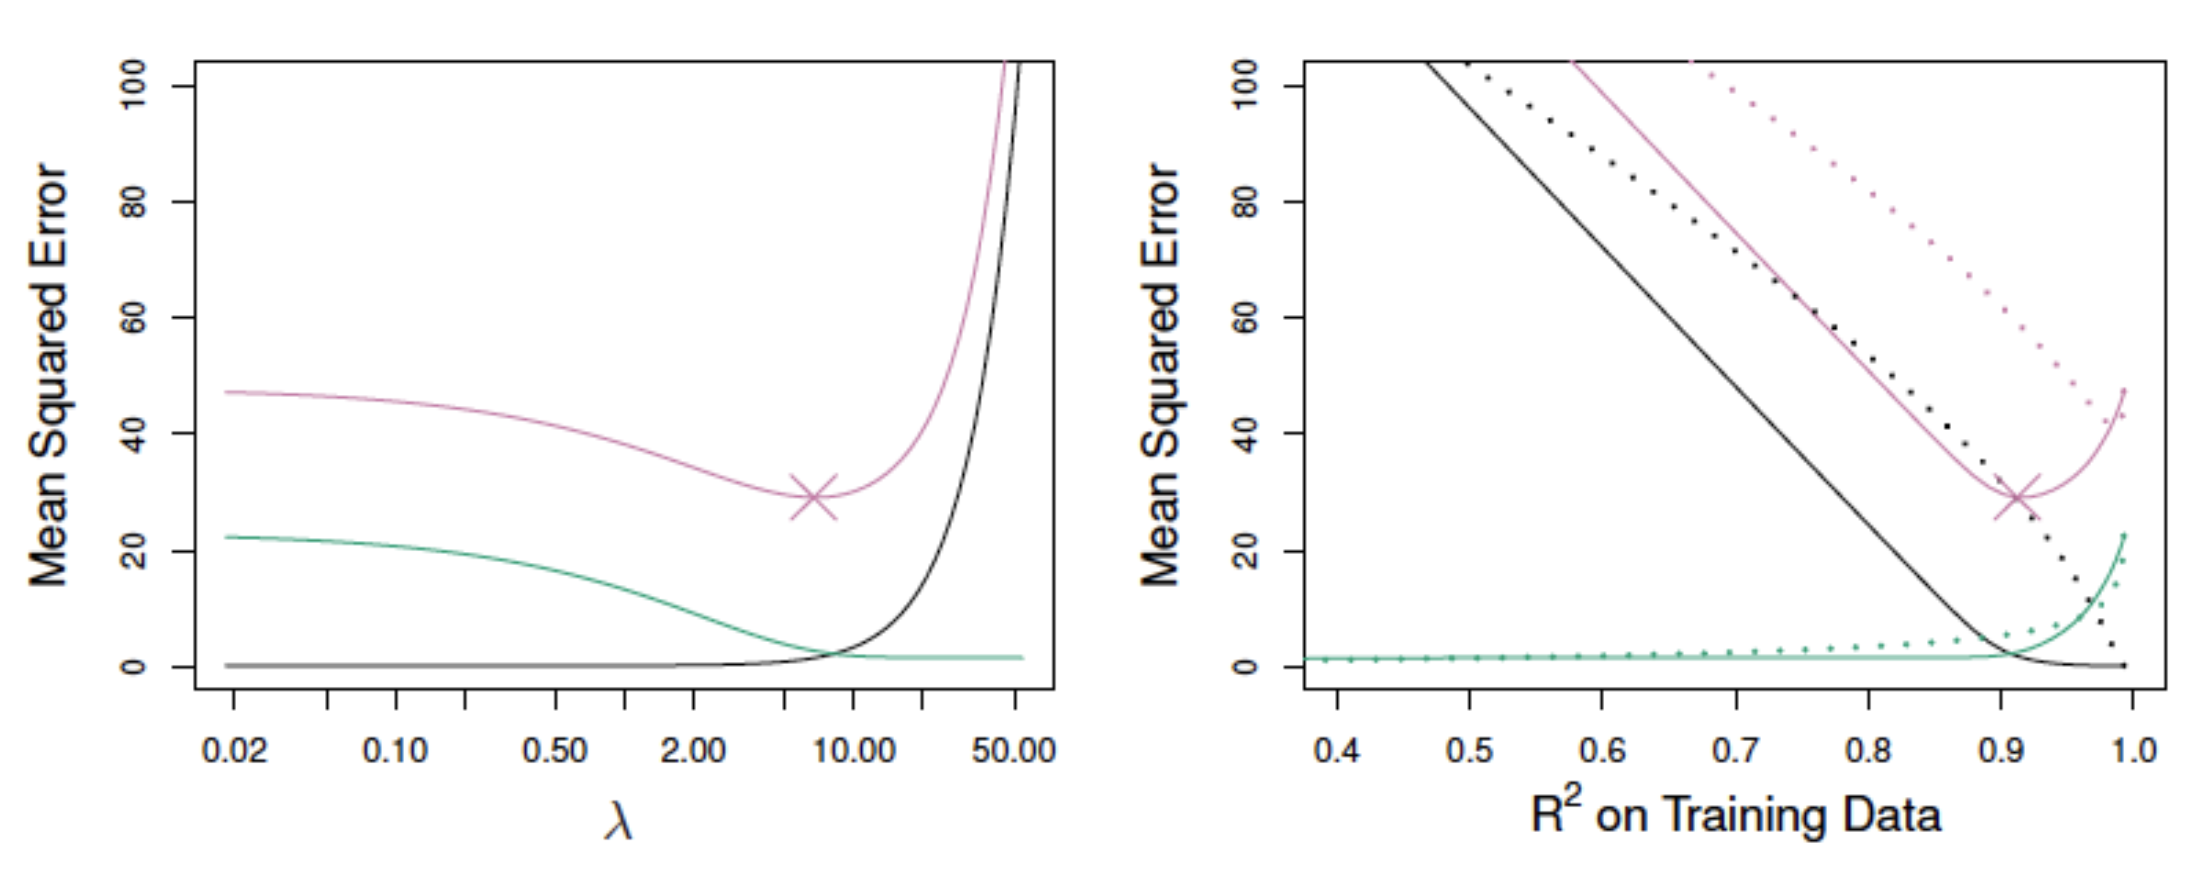
\includegraphics[width=0.8\linewidth]{./figures/chapter_4/lassoridgecomparison2.png}
    \caption{Comparison between lasso and ridge regression with a small number of predictors. \textcolor{green}{Green} curve represents the variance, black curve represents the bias and the \textcolor{red}{red} curve represents the test mean squared error.}
    \label{fig:lassoridgecomparison2}
\end{figure}

For equity, we now consider a case where the response is actually a function of only $2$ out of $45$ predictors by analyzing the figure \ref{fig:lassoridgecomparison2}. We can see that the lasso is way better than ridge regression for every component of the MSE.

These two examples allow us to understand how neither lasso nor ridge regressions represent a universal solution. In general, we might expect lasso to perform better in settings where only a small number of predictors have substantial coefficients, the remainder approaching zero. Conversely, ridge regression will perform better when the response is a function of many predictors, with similar average coefficients.
However, the amount of predictors that are actually related to the response is never known to prori for real datasets. Thus, a technique such as cross-validation can be used in such a way as to determine which approach is best for a particular dataset.

% In order to compare lasso and ridge regression, let's consider the case in which we have $p=45$ and $n=50$. The first plot shows the mean squared error and its components for lasso regression. We can see that the behaviour is similar to that of the ridge regression but for large values of $\lambda$, the mean squared error converges to a fixed value that is because \textbf{??}.

% The second plot shows a comparison between lasso and ridge in terms of mean squared error, with $R^2$ as independent variable. We can see that while the bias curves are almost identical, the variance of ridge is slightly lower than the variance of lasso and this makes ridge regression better than lasso in this particular case.

% This happened because all the 45 predictors were truly related to the response, and none of the true coefficients were actually equal to zero. Let us now consider the case where the response is actually a function of only $2$ out of $45$ predictors. The second plot shows that the lasso is way better than ridge regression for every component of the MSE.

% From this, we can derive that there is no best approach between ridge or lasso regression, since lasso tends to perform better in a setting only a small number of predictors have substantial coefficients; while ridge regression will perform better when the response is a function of many predictors. But since we don't have this information \textit{a priori} in real cases, we can use the cross validation approach to determine which approach is better on a particular dataset. Additionally, an advantage of lasso is the fact that the models are sparse and thus easier to interpret.

\subsubsection*{A special case for Ridge Regression and the Lasso}
In such a way as to better understand the intuition behind the behavior of the ridge regression and lasso methods, let us consider a special case.
Let's assume that:
\begin{itemize}
    \item $\underline{\underline X}$ is an \textbf{orthonormal matrix} 
    \item $n=p$
    \item $\beta_0 = 0$, so that there is no intercept
\end{itemize}

\[
    \underbar{\underbar X} = \begin{bmatrix}
        1 & 0 & \dots & 0 \\
        0 & 1 & \dots & 0 \\
        \vdots & \vdots & \ddots & \vdots \\
        0 & 0 & \dots & 1
        \end{bmatrix}\text{ Orthonormal Squared Matrix}
\]

In this special case it can be shown that the three procedures have explicit solutions. Let $\hat{\beta}_j$ be the OLS estimate of $\beta_j$.

With these assumptions, the OLS estimate procedure can be reconducted to the minimization of the quantity:
\[
    \sum_{j=1}^p \left(y_j - \beta_j\right)^2 
\]

The straightfoward solution is that
\[
    \hat{\beta}_j = y_j
\]

While, for the ridge regresssion, the problem is to minimize the quantity:
\[
    \sum_{j=1}^p \left(y_j - \beta_j\right)^2 + \lambda \sum_{j=1}^p \beta_j^2
\]

Instead, for lasso:
\[
    \sum_{j=1}^p \left(y_j - \beta_j\right)^2 + \lambda \sum_{j=1}^p |\beta_j|
\]

It can be shown that, in this special case, the ridge regression estimate is given by:
\[
    \hat{\beta}^{R} = \left(\underline{\underline X}^T \underline{\underline X} + \lambda I\right)^{-1} \underline{\underline X}^T y = \hat{\beta}_j^R = \frac{\hat{\beta}_j}{1 + \lambda}
\]

While the lasso estimate is given by:
\[
    \hat{\beta}_j^L = \text{sign}(\hat{\beta}_j)\left(|\hat{\beta}_j| - \frac{\lambda }{2}\right)_+
\]
where:
\[
    x_+ = \begin{cases}
        x\quad\text{if $x > 0$}\\
        0\quad\text{if $x\le 0$}
        \end{cases}
\]

For a best subset selection of size $s$ the solution is:
\[
    \hat{\beta}_j^B = \hat{\beta}_j \cdot I(|\hat{\beta}_j| \geq |\hat{\beta}_{(s)}|)
\]
where $|\hat{\beta}_{(s)}|$ is the $s$-th largest among all $|\hat{\beta}_j|$.






This allows us to make another comparison between ridge regression, lasso and the best subset selection approach:
\begin{itemize}
    \item ridge regression does a \textbf{proportional shrinkage} of OLS estimates of a factor of $1+\lambda$
    \item lasso translates each coefficient by a constant factor $\frac{\lambda}{2}$; if the coefficients are lower thant $\frac{\lambda}2$ they will be truncate at zero (and this explain also the variable selection property). So it performs a \textbf{soft-thresholding}.
    \item best subset selection drops all variables with coefficients smaller than the $s$-th largest, this is a form of \textbf{hard-thresholding}.
\end{itemize}

In the general case, where the previous assumptions are not satisfied, the history is a bit more complicated but the main ideas are the same.
% slide 20 plots

Now, we want to prove the previous result on the ridge regression coefficients.
\paragraph*{Proposition}
The coefficients of the ridge regression are:
\[
    \hat{\beta}^{ridge} = \left(X^T X + \lambda I\right)^{-1} X^T y
\]
and they can be rewritten as:
\[
    \hat{\beta}_j^R = \frac{\hat{\beta}_j}{1 + \lambda}
\]


\paragraph*{Proof}
We start by solving the following problem:
\[
    \hat{\beta}_{ridge} = \arg\min_\beta  \left\{ \sum_{i=1}^n (y_i - \beta_0 - \sum_{j = 1}^p \beta_j x_{ij})^2  + \lambda\sum_{j = 1}^p \beta_j^2 \right\} = \arg\min_\beta \text{RSS}^{\prime} (\beta)
\]
\callout{Note}{Note that this can be generalized by considering a penalty term $\lambda \sum_{j=1}^p|\beta_j|^q$.}
Firstly we need to standardize the data points:
\[
    x_{ij} \to \frac{x_{ij} - \overline{x}_j}{\sigma_j}
\]
Note that $\beta_0 = \overline{y}$. So we consider $y_i - \overline{y}$. Instead of having a design matrix with $p+1$ columns, we use $p$ columns by dropping $\beta_0$.

Then we need to find $\hat{\beta}_{ridge}$ by minimizing $\text{RSS}'(\beta, \lambda)$. We now compute the gradient of $\text{RSS}^{\prime}$ wrt $\beta$ and then equate it to zero.
\[
    \nabla_\beta \text{RSS}^{\prime} (\beta, \lambda) = 0
\]
By considering standardization we have the following dimensions:
\begin{align*}
    X: n\times p     \\
    \beta: p\times 1 \\
    Y: n \times 1
\end{align*}
We now rewrite $\text{RSS}^{\prime}$ in matrix form:
\begin{align*}
    \text{RSS}^{\prime} & = (Y - X \beta)^T (Y - X \beta) + \lambda \beta^T \beta =                                                                                              \\
                        & = Y^T Y - \underbrace{\beta^T X^T Y}_{scalar} - \underbrace{Y^T X \beta}_{scalar}+                 \beta^T X^T X \beta + \lambda I_{p} \beta^T \beta = \\
                        & = Y^T Y - 2 \beta^T X^T Y + \beta^T (X^T X + \lambda I_p) \beta
\end{align*}

Now we can compute $\nabla_\beta \text{RSS}^{\prime} $. The derivative of $Y^T Y$ is zero, the derivative of $- 2 \beta^T X^T Y $ is $- 2 X^T Y $ and finally the derivative of $\beta^T (X^T X + \lambda I_p) \beta$ is composed by two main terms but since the matrix is simmetric ($(X^TX+\lambda I_p)^T=(X^TX)^T+(\lambda I_p)^T=(X^TX+\lambda I_p)$) is equal to the sum of the two terms $2(X^T X + \lambda I_p) \beta$. So we get:
\[
    \nabla_\beta\text{RSS}^{\prime} = - 2X^T Y + 2(X^T T + \lambda I_p) \beta = 0
\]
The solution of this equation is:
\[
    \hat{\beta}_{ridge} = (X^T X + \lambda I)^{-1} X^T Y
\]
Let us now consider the $\hat{\beta}_{OLS}$ estimator:
\[
    \hat{\beta}_{OLS} = (X^T X)^{-1} X^T Y
\]
The two solutions are similar. 
The main difference is that the ridge regression estimator has a positive quantity on the diagonal of the matrix $X^T X$.
We remember that the matrix $X^T X$ is an estimator of the \textbf{variance-covariance matrix}.
Adding a positive quantity on its primary diagonal helps us to increase the determinant of the matrix. This helps to invert the matrix and balance the problem of \textit{collinearity} where, in that circumstance, tends to have a variance-covariance matrix near to singularity.

In case of \textbf{orthonormal inputs} ($n \geq p$):
\[
    X^T X = I_p \qquad \text{Condition of Orthonormality}
\]

The previous \textbf{Condition of Orthonormality} is satisfied when the columns of the matrix $X$ are \textbf{orthonormal}. 
In algebra, if $n = p$ the condition of orthonormality can also be written as $X^T = X^{-1}$; while if $n > p$ the condition is $X^T X = I_p$ (\textit{pseudoinverse}).

If we apply the previous condition to the OLS and Ridge estimators, we get:
\begin{gather*}
    \hat{\beta}_{OLS} = (X^T X)^{-1} X^T Y = I_p^{-1} X^T Y = X^T Y \\
    \hat{\beta}_{ridge} = (X^TX + \lambda I_p)^{-1}X^T Y = (I_p + \lambda I_p)^{-1} X^T Y = \frac{I_p}{1+\lambda} \hat{\beta}_{OLS}
\end{gather*}

The same approach works also for lasso.

\section{PCA}
\textbf{Principal Component Analysis} is a linear transformation that projects the data onto the space.
The feature space is described in terms of the principal components, also named \textbf{principal directions}. PCA has the following characteristics:
\begin{itemize}
    \item the transformed features are linearly uncorrelated
    \item the first transformed feature has the highest variance among the others, the second transformed feature has the second highest variance among the others, and so on...
    \item If our features indicated something like the temperature, the pressure and so on, then after projecting them onto the new space, they will lose that meaning.
    \item By considering a subset of the principal directions in the new space, we are able to perform \textbf{dimensionality reduction}.
\end{itemize}

An example of transformation is the Fourier transform, that maps all the samples of a sinusoidal function into one single features that represents the frequency. In this case, the \textit{base} of the space in which we want to project the new features is known, but in the principal component analysis case we need to learn first the \textit{bases} of the new space from the data.

\subsubsection*{The rationale}
By representing the data onto a new space, the PCA allows us to get a representation characterized by having the \textit{lowest projection distance} and so by . 
The principal components of the new space are simply a linear combination of the feature in the original dataset.

After the projection, the \textbf{variance} of the data is preserved. This means that the information contained is preserved. Also the feature with the highest variance will be the first principal component, and so on. In this way we are able to discard the least important features and works in a space with $k\le p$ dimensions.

\subsection{Construction}
Assume we have a dataset $X^{\prime} \in \mathbb{R}^{n \times p}$. A preliminary thing to do is to center the dataset by subtracting the mean $\mu$ of each feature from the corresponding feature.
\[
    \mu = \frac{1}{n} \sum_{i = 1}^{N} x^{\prime}_i
\]
\[
    X = \begin{bmatrix}
        x^{\prime}_1 - \mu_1 \\
        x^{\prime}_2 - \mu_2 \\
        \vdots               \\
    \end{bmatrix}
\]
Principal Component Analysis is simply the application of the following linear transformation:
\[
    T = X W
\]
where $W \in \mathbb{R}^{p \times p}$ is the projection matrix which contains the \textbf{principal directions} as columns and $T \in \mathbb{R}^{n \times p}$ are the \textbf{principal components} of $X$, i.e. the new representation of $X$ in the space described by the principal directions. By construction, we assume that the principal directions are orthonormal, i.e. $W^T W = I$.

Each row of $X$ is a sample of the dataset, each column of $W$ is a principal direction, so the dot product between a row of $X$ and a column of $W$ is the projection of the sample onto the principal direction. In other words, By mutiplying $X$ by $W$ we are applying the dot product on each feature, thus projecting each feature onto the principal directions.

\subsubsection*{Building $W$}
Now we want to understand how do we obtain the matrix $W$. We know that the \textbf{first} column of $T$ should have the highest variance among the others. So we will need to solve the following optimization problem:
\[
    w^{(1)} = \arg \max_{\omega \in \mathbb{R}^p} \left\{\frac{1}{n-1} \sum_{i = 1}^{n} \left(\sum_{i = 1}^{p} x_{ij} \omega_j \right)^2\right\} \quad \text{s.t.} \|w\|^2 = 1
\]
This problem is constrained by the fact that the norm of $w$ must be equal to $1$ because we impose that the principal directions are orthonormal.

Note that the inner sum is the dot product between the $i$-th sample and the respective principal direction $w$ so it gives us the squared sum of the principal components, which averaged for the number of samples gives us the variance of the $j$-th principal component (recall $x$ is zero-mean because we scaled the features).
So, the optimization problem is searching for the vector $\omega$ that maximizes the variance of the principal component calculated (on some books called \textbf{PC score}).

Rewriting the problem in matrix notation:
\[
    w^{(1)} = \arg \max_{\omega \in \mathbb{R}^p} \|X\omega\|^2 = \arg \max_{\omega \in \mathbb{R}^p} \left(\omega^T X^T X \omega\right)\quad \text{s.t.} \|w\|^2 = 1
\]
We can consider the assumption of orthonormality inside the expression:
\[
    w^{(1)} = \arg \max_{\omega \in \mathbb{R}^p} \left(\frac{\omega^T X^T X \omega}{\omega^T \omega}\right) %\quad \text{s.t.} \|w\|^2 = 1
\]
The function we want to maximize is well known as \textbf{Rayleigh quotient} and is know that if $X^T X$ is a positive semi-defined matrix then the Rayleigh quotient is maximized by \textbf{the eigenvector corresponding to the largest eigenvalue} of $X^T X$.
Since we know that $X^T X$ is an estimate of the covariance matrix of $X$, we know that it is a positive semi-defined matrix, so we can apply the result.

Now in order to find the other principal directions (aka, the other columns of $W$) we first need to find the orthogonal part of the projection, by projecting the data onto the space spanned by the first principal direction and then subtracting the projection from the data. We can visually understand this by looking at the figure \ref{fig:orthogonal_projection}.

\begin{figure}
    \centering
    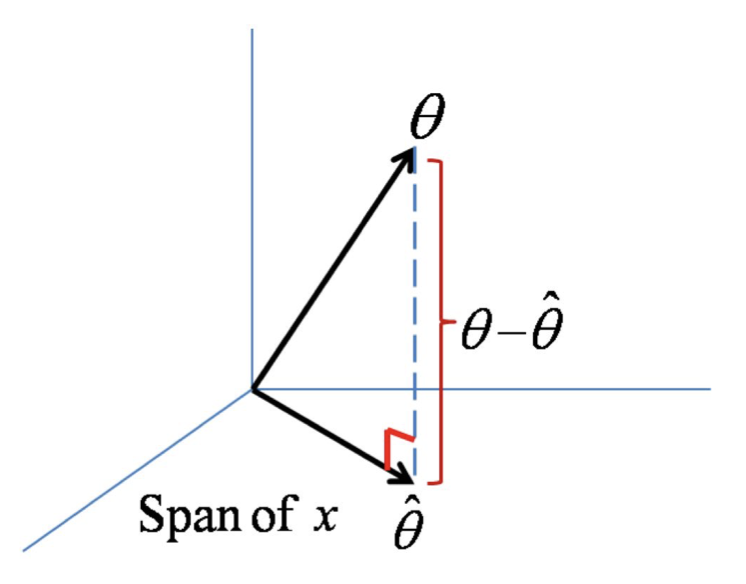
\includegraphics[width=0.5\textwidth]{./figures/chapter_7/orthogonal_projection.png}
    \caption{Orthogonal projection of the data onto the space spanned by the first principal direction.}
    \label{fig:orthogonal_projection}
\end{figure}

In general, to obtain the projection onto the first $k-1$ directions, we can perform this projection by applying the following transformation:
\[
    X_k = X - X \underbrace{\sum_{i=1}^{k-1} w^{(i)} w^{(i)T}}_{\text{Orthogonal projection matrix}}
\]
Where $k$ is the number of the principal direction we want to compute.  We can now apply the same procedure as before to find the $k$-th principal direction. Then, as a generalization of the previous result, it can be shown that the $k$-th principal direction is the eigenvector corresponding to the $k$-th largest eigenvalue of $X^T X$.

To sum up we've shown that the principal directions are the eigenvectors of the covariance matrix $X^T X$ and the principal components are the eigenvectors associated to the largest eigenvalues of $X^T X$. 

\[
    \omega^{(k)} = \arg \max_{\omega \in \R^p} \left(\frac{\omega^T X_k^T X_k \omega}{\omega^T \omega}\right)
\]

Finally, we found that $W$ is the matrix whose columns are the eigenvectors of $X^T X$ sorted by the eigenvalues in decreasing order.

\subsubsection*{Data Covariance Matrix}
As we've said, $X^TX$ is an estimate of the covariance matrix of $X$. In particulr, the covariance matrix of $X$ is a $p\times p$ matrix defined as:
\[
    C = \frac{1}{n-1} \sum_{i=1}^n x_i^T x_i = \frac{1}{n-1} X^T X
\]
Since its columns are the \textit{principal directions} of the new space, we can show that the corresponding eigenvalues are the variances of the principal components (i.e. of the data projected onto the principal directions).
%We will now show that the eigenvalues are the variances of each principal component. 
Let us consider the first eigenvalue, by definition of eigenvalue and eigenvector we have:
\[
    \underset{\text{Property of eigenvalues}}{A u^{(k)} = \lambda_k u^{(k)}} \implies X^T X \omega^{(1)} = \lambda_1 \omega^{(1)}
\]
Multiplying both sides by $(w^{(1)})^T$ we get:
\[
    (\omega^{(1)})^T X^T X \omega^{(1)} = \lambda_1 \omega^{(1)}(\omega^{(1)})^T \implies \|X \omega^{(1)}\|^2 = \lambda_1 \|\omega^{(1)} \|^2 \underset{\|\omega^{(1)}\|^2=1}= \lambda_1
\]
Then by definition of variance we have:
\[
    \text{Var}\left[X \omega^{(1)}\right] = \frac{1}{n-1} \|X \omega^{(1)}\|^2 = \frac{\lambda_1}{n-1}
\]
So we have shown that the eigenvalues of $X^T X$ are (proportional to) the variances of the principal components.

\subsubsection*{Uncorrelation}
Another characteristics of the principal component analysis is that it \textit{gives us uncorrelated data} in the new space. To show this, let us consider the covariance matrix of the principal components:
\[
    \frac{T^T T}{n-1} = \frac{W^T X^T X W}{n-1} \overset{\text{ED}}= \frac{W^T W \Lambda W W^T}{n-1} = \frac{\Lambda}{n-1}
\]
First we used the fact that $X^T X$ is similar to $W \lambda W^T$ since now we know that the columns of $W$ are the eigenvectors of $X^TX$, then we've used the fact that $W^T W = I$ because we imposed orthogonality.
So we have shown that the covariance matrix of the principal components is a diagonal matrix, which means that all the covariances are zero, i.e. the principal components are uncorrelated.

\subsection{Dimensionality Reduction}
We can use PCA to select only a subset of size $m$ of the principal components, thus reducing the dimensionality of the data. We can do this by selecting the first $m$ columns of $T$.

In this way we are selecting the $m$ principal component that explain the most variance of the data. We can compute the \textbf{percentage of variance explained} or \textbf{PVE} by the $m$ principal components as:
\[
    PVE = \frac{\sum_{k=1}^m \lambda_k}{\sum_{j=1}^p \lambda_j}
\]
% something about the rank of the covariance matrix 

The main drawback of applying PCA is that we are losing the meaning of the features (explainability), so we are not able to interpret the data anymore.

\subsection{Singular Value Decomposition}
\textbf{Singular Value Decomposition} is a generalization of the eigenvalue decomposition for rectangular matrices and is the effectively technique used in the software. 

Let us consider a matrix $M \in \mathbb{R}^{n \times p}$, that we can decompose it as:
\[
    M = U \Sigma V^T
\]
where $U \in \mathbb{R}^{n \times n}$ and $V \in \mathbb{R}^{p \times p}$ are \textbf{orthogonal} matrices respectively called \textbf{left singular vectors} and \textbf{right singular vectors}, while $\Sigma \in \mathbb{R}^{n \times p}$ is a \textit{rectangular diagonal}\footnote{Is simply a couple of adjective to indicate a rectangular matrix that has a subdiagonal (not a complete diagonal) and all other values to $0$.} matrix with the \textbf{singular values} of $M$. 

In particular, the number $r$ of non-zero singular values is equal to the rank of $M$.

Since the elements under the diagonal of $\Sigma$ are zero, we can cut the matrix to simplify the calculations and obtain a matrix $\Sigma\in \R^{r\times r}$.

\subsubsection*{PCA with SVD}
If we decompose $X$ as $X = U \Sigma V^T$ then we can rewrite the covariance matrix as:
\[
    X^T X = (U \Sigma V^T)^T U \Sigma V^T = V \Sigma^T U^T U \Sigma V^T = V \Sigma^T \Sigma V^T
\]
because $U$ is defined as an orthogonal matrix, so $U^T U = I$.
So we found out that the covariance matrix of $X$ is similar to $\Sigma^T \Sigma$ and we know that similar matrices have the same eigenvalues.

If we call $\sigma_i$ the $i$-th singular value of $X$ then we have that $\sigma_i^2$ is equal to the $i$-th eigenvalue of $X^T X$.

The project dataset is simply obtained using as \textit{transformation matrix} a matrix of singular vectors:
\[
    T = X V = U \Sigma V^T V = U \Sigma
\]

As we've done for the eigenvalue decomposition, we can use the first $m$ columns of $T$ to perform dimensionality reduction.
